\documentclass[12pt]{article}

%==============Packages & Commands==============
\usepackage{graphicx}
\usepackage{fancyvrb}
\usepackage{tikz}
%%%<
\usepackage{listings}
%\usepackage[active,tightpage]{preview}
%\PreviewEnvironment{tikzpicture}
%\setlength\PreviewBorder{5pt}%

\usepackage{geometry}                		% See geometry.pdf to learn the layout options. There are lots.
\geometry{letterpaper}                   		% ... or a4paper or a5paper or ...
%\geometry{landscape}                		% Activat\usetikzlibrary{arrows}e for for rotated page geometry
%\usepackage[parfill]{parskip}    		% Activate to begin paragraphs with an empty line rather than an indent
\usepackage{graphicx}				% Use pdf, png, jpg, or eps§ with pdflatex; use epFs in DVI mode
								% TeX will automatically convert eps --> pdf in pdflatex
\usepackage{amsmath}
\usepackage{amssymb}

%\usepackage[ruled,vlined]{algorithm2e}
\usetikzlibrary{arrows}
\usepackage{alltt}
\usepackage[T1]{fontenc}
%\usepackage[utf8]{inputenc}
\usepackage{indentfirst}
\usepackage[longnamesfirst]{natbib} % For references
\bibpunct{(}{)}{;}{a}{}{,} % Reference punctuation
\usepackage{changepage}
\usepackage{setspace}
\usepackage{booktabs} % For tables
\usepackage{floatrow}
\usepackage{rotating} % For sideways tables/figures
\usepackage{amsmath}
\usepackage{multirow}
\usepackage{color}
 
\definecolor{codegreen}{rgb}{0,0.6,0}
\definecolor{codegray}{rgb}{0.5,0.5,0.5}
\definecolor{codepurple}{rgb}{0.58,0,0.82}
\definecolor{backcolour}{rgb}{0.95,0.95,0.92}
 
\lstdefinestyle{mystyle}{
    backgroundcolor=\color{backcolour},   
    commentstyle=\color{codegreen},
    keywordstyle=\color{magenta},
    numberstyle=\tiny\color{codegray},
    stringstyle=\color{codepurple},
    basicstyle=\footnotesize,
    breakatwhitespace=false,         
    breaklines=true,                 
    captionpos=b,                    
    keepspaces=true,                 
    numbers=left,                    
    numbersep=5pt,                  
    showspaces=false,                
    showstringspaces=false,
    showtabs=false,                  
    tabsize=2
}
 
\lstset{style=mystyle}
\usepackage{dcolumn}
\usepackage{comment}
%\usepackage{fullwidth}
\newcolumntype{d}[1]{D{.}{\cdot}{#1}}
\newcolumntype{.}{D{.}{.}{-1}}
\newcolumntype{3}{D{.}{.}{3}}
\newcolumntype{4}{D{.}{.}{4}}
\newcolumntype{5}{D{.}{.}{5}}
\usepackage{float}
\usepackage[hyphens]{url}
%\usepackage[margin = 1.25in]{geometry}
%\usepackage[nolists,figuresfirst]{endfloat} % Figures and tables at the end
\usepackage{subfig}
\captionsetup[subfloat]{position = top, font = normalsize} % For sub-figure captions
\usepackage{fancyhdr}
%\makeatletter
%\def\url@leostyle{%
%  \@ifundefined{selectfont}{\def\UrlFont{\sf}}{\def\UrlFont{\small\ttfamily}}}
%\makeatother
%% Now actually use the newly defined style.
\urlstyle{same}
\usepackage{times}
\usepackage{mathptmx}
%\usepackage[colorlinks = true,
%						bookmarksopen = true,
%						pagebackref = true,
%						linkcolor = black,
%						citecolor = black,
% 					urlcolor = black]{hyperref}
%\usepackage[all]{hypcap}
%\urlstyle{same}
\newcommand{\fnote}[1]{\footnote{\normalsize{#1}}} % 12 pt, double spaced footnotes
\def\citeapos#1{\citeauthor{#1}'s (\citeyear{#1})}
\def\citeaposs#1{\citeauthor{#1}' (\citeyear{#1})}
\newcommand{\bm}[1]{\boldsymbol{#1}} %makes bold math symbols easier
\newcommand{\R}{\textsf{R}\space} %R in textsf font
\newcommand{\netinf}{\texttt{NetInf}\space} %R in textsf font
\newcommand{\iid}{i.i.d} %shorthand for iid
\newcommand{\cites}{{\bf \textcolor{red}{CITES}}} %shorthand for iid
%\usepackage[compact]{titlesec}
%\titlespacing{\section}{0pt}{*0}{*0}
%\titlespacing{\subsection}{0pt}{*0}{*0}
%\titlespacing{\subsubsection}{0pt}{*0}{*0}
%\setlength{\parskip}{0pt}
%\setlength{\parsep}{0pt}
%\setlength{\bibsep}{2pt}
%\renewcommand{\headrulewidth}{0pt}

%\renewcommand{\figureplace}{ % This places [Insert Table X here] and [Insert Figure Y here] in the text
%\begin{center}
%[Insert \figurename~\thepostfig\ here]
%\end{center}}
%\renewcommand{\tableplace}{%
%\begin{center}
%[Insert \tablename~\theposttbl\ here]
%\end{center}}

\newcommand\independent{\protect\mathpalette{\protect\independenT}{\perp}}
\def\independenT#1#2{\mathrel{\rlap{$#1#2$}\mkern2mu{#1#2}}}
\newcommand{\N}{\mathcal{N}}
\newcommand{\Y}{\bm{\mathcal{Y}}}
\newcommand{\bZ}{\bm{Z}}

\usepackage[colorlinks = TRUE, urlcolor = black, linkcolor = black, citecolor = black, pdfstartview = FitV]{hyperref}


%============Article Title, Authors==================
\title{\vspace{-2cm} Network Effects in Field Experiments on Interactive Groups: Cases from Legislative Studies } 


\author{Sayali Phadke \thanks{\footnotesize{PhD Student, Departments of Statistics, Pennsylvania State University, sayalip@psu.edu.}} \and Bruce A. Desmarais \thanks{\footnotesize{Associate Professor, Department of Political Science, Pennsylvania State University, bdesmarais@psu.edu.}}} \date{\today}



%===================Startup=======================
\begin{document}
\maketitle



%=============Abstract & Keywords==================

\begin{abstract} 
\vspace{.3cm}
\begin{center}
{\bf DRAFT, RESULTS MAY CHANGE}
\end{center}
\vspace{.3cm}

\noindent  Most social processes involve complex interaction among units through some form of social, communication, or collaboration network. The stable unit treatment value assumption (SUTVA)---the assumption that a unit's outcome is unaffected by other units' treatment statuses---is required in conventional approaches to causal inference. When SUTVA is violated, as in networked social interaction, treatment effects spread to control units through the network structure. We evaluate the evidence for spillover effects in data from three field experiments on US state legislatures. Randomized field experiments represent the gold standard in causal inference when studying political elites. It is rarely possible to bring political elites into a controlled laboratory environment, and causal identification with observational data is fraught with problems. We review recently-developed methods for testing for causal effects---including interference effects---while relaxing SUTVA. We propose new specifications for treatment spillover models, and construct networks through geographical or ideological proximity and co-sponsorship. Considering different combinations of spillover models and networks, we evaluate the robustness of recently developed non-parametric tests for interference. The approaches we illustrate can be applied to any experimental setting in which interference is suspected.\footnote{Prepared for presentation at the 2016 Political Networks Conference, Washington University, St. Louis. Work supported in part by National Science Foundation grants SES-1558661, SES-1619644, CISE-1320219, and IGERT Grant DGE-1144860, Big Data Social Science. Any opinions, findings, and conclusions or recommendations are those of the authors and do not necessarily reflect those of the sponsor.} 
\\~\\~\\
\end{abstract}

\thispagestyle{empty}
\doublespacing


\section{To-do before submission}
\begin{itemize}

\item A note on why the adjustment for expected exposure in Coppock's method is not critical [BD]

\item A note explaining the intuition behind the meaning of movement in effect estimate due to spillover specification. Depending upon the context, estimate under SUTVA is either conservative or or optimistic. In some cases, effect spilling over to neighbors is good (GOTV mails). In others, it is may show that the treatment has worked worse than we thought (disease prevention). This may also depend upon the type of network being used (e.g. friendship network v/s enmity network). This leading into a note about SUTVA violations resulting in attenuation bias (example: Ghana experiment) [BD]

\item A note that we are not distinguishing between contagion and spread of treatment itself, at this point [BD]

\item A note on interpretation of CIs. Can we explain them in terms of 'if 100 such tests were conducted, 95\% of the p-values would lie in this interval' [SP\&BD]

\item Include geographical network in Coppock and Bergan [SP][Can't find the code used to generate Coppock geographical net]

\item Consider additional test statistic such as the Anderson-Darling test and other tests mentioned in \citep{rosenbaum2012interference} (Mann-Whitney U test, Control Median test etc.) [SP]

\item Consider weighted combinations of different networks to estimate a $\gamma$ [Maybe; SP]

\item Do we want to include network plots for all networks we have considered? [Could look into local egocentric networks; however this is low priority]

\item Separate out the high and low support district in original data and conduct separate analyses. This would explain the direction of the spillover effect much better. Conduct this analysis with ideological network as well as committee network [Low priority: SP]

\item Explore the idea of using communities to model spread across the network [Lower priority]

\end{itemize}


%%%%
% Description of the possible challenges
\section{Introduction}
%%%%

In social science, researchers often focus on sets of actors who interact on a regular basis. Areas of social science research in which regular and familiar interaction constitutes the norm include the study of team performance in formal organizations \citep[e.g., ][]{anderson1992}, the study of students from the same school/classroom \citep[e.g., ][]{sallis1997}, and the study of political elites from the same political institution \citep[e.g.,][]{bratton1999}. The importance of collections of highly interactive individuals, which may have conventionally been termed ``small groups.'' \citep{levine1990}, spans disciplines; including social psychology, public health, political science and organizational studies. Given the rise of research focused on social media \citep{agichtein2008}, which includes the study of interpersonal interaction, but is focused on large groups, we will use the term, ``interactive group research.'' 

To draw causal inferences in the study of an interactive group, the most reliable approach is to run a randomized experiment in which the researcher controls one or more interventions. Due to the interactions between group members, the effect of an intervention on one group member may spread to others through the network of interactions. The conventional framework for causal inference relies on SUTVA (Stable Unit Treatment Value Assumption). SUTVA holds that one unit/subject is not affected by the treatment status of any other unit \citep{sekhon2008}. However, SUTVA breaks down in a network setting \citep{galea2010} when there are post-treatment interactions among units. The violation of SUTVA is termed ``interference''.  When testing for causal effects in experiments on interactive groups, there are two related motivations for researchers to test and account for interference. First, even if the researcher is not interested in the nature of interference, it may be necessary to account for interference to accurately identify the direct effects of interventions on units. Second, interference processes may play a major role in shaping individual or group outcomes, and may therefore be important to evaluate if the objective of the research is to understand or explain outcomes arising from the group's social process. 

Social influence and other processes of interdependence are central to nearly every domain of social science, researchers are well aware of the major limitations associated with causal inferences regarding influence drawn from observational studies \citep{Shalizi:2011}. As such, a growing body of research seeks to study interference through experimental interventions \citep[e.g., ][]{gerber2008,paluck2011,Bond:2012,muchnik2013,aral2014,bapna2015,Ben-AaronPAR}. These studies follow a variety of approaches to designing the interventions and testing for interference effects. However, it is clear that the field has, as of yet, converged upon a consistent methodological framework for testing for causal effects in the presence of interference.  

We review a recently developed general framework, introduced by \citet{bowers2012reasoning}, for testing causal hypotheses in the presence of interference. As an illustration, we then apply this methodology to data generated by field experiments on US state legislatures \citep{butler2011can,bergan2015call}; experiments that were not intended to study interference. As part of our application, we discuss and illustrate several choices researchers need to make in testing interference hypotheses.

Our results are three-fold. First, we review a broad framework for evaluating interference hypotheses, and make the case that researchers should consider such hypotheses when evaluating the results of experiments on interactive groups. Second, we show that we consistently find evidence in support of interference hypotheses in data from field experiments on US state legislatures. Third, we encourage researchers to consider several modeling dimensions in formulating interference hypotheses.


%\section{Background}

%\begin{itemize}
%\item Paragraph on each category of papers that serve as relevant background (SP)
%\item Interference models (diffusion, propagation) (SP--Review)
%\item  Experiments on networks (applications) (SP--Review)
%\item Approaches to inference or estimation with propagation (SP--Review) 
%\item Potential outcomes framework (SP -- find papers \& Review)
%\item Review of political networks (SP--Review)
%\item Review of field experiments (SP--Review)
%\begin{itemize}
%\item \citep{Gottlieb:2015,Alatas:2012,Kalla:2015, Malesky:2012,Ichino:2012,Nyhan:2014}
%\end{itemize}
%\end{itemize}


%%%%
\section{Experimental Research on Interactive Groups}
%%%%

%%%% Field experiments are often the most externally valid, and permit causal identification, also can be the only option if researching elites.

In laboratory experiments, especially those in which the treatment is administered and response measured while the subject is in the lab, it is feasible to assure that subjects do not interact, such that SUTVA holds. However, in administering laboratory experiments with the intent of generalizing results to a target population of interest, researchers face the dual tasks of (1) recruiting participants from a target population of interest and (2) recreating real-world conditions relevant to the effects of the treatment. Since it is often impossible to complete these tasks, laboratory experiments often suffer from a lack of external validity, where external validity is understood to be the generalizability of the effects of the treatment in the laboratory to members of the target population outside of the lab setting. \citet[p.245]{lucas2003} puts it concisely, ``Laboratory experiments are considered externally invalid because findings from the population studied cannot be generalized to populations other than the one from which the sample was drawn.'' This quote is an over-simplification, but it underscores the advantage of field experiments relative to lab experiments. That is, field experiments are directed at the population of interest, in its natural setting \citep{list2014field}. 

One characteristic of field experiments is that the researchers cannot prevent subjects from interacting. Furthermore, we argue, several classes of field experiments are conducted within contexts that are likely to lead to interaction among subjects. Such interaction should lead to the possibility that the results of the experiment reflect the effects of the experimental conditions to which subjects were assigned, as well ass interference across subjects according to patterns of interaction. 

The first class of field experimental designs we discuss involves experimenting on relatively small groups of subjects who work for the same organization, in either the same building or on the same campus. Examples from this class include \citet{hennig2010search}, who studied the work-effort effects of presenting comparative pay information to student workers at a single university; \citet{grant2007impact}, who studied the effects on motivation of having employees in a fundraising organization interact with the organization's beneficiaries; and \citet{jackson1983participation}, who, looking at nurses and clerical staff in a single hospital, studied the effects of employee participation in decision making on several factors associated with employees' perceptions of their roles in and influence on the hospital's operations. These experiments present the ideal conditions for interference, since these experiments involve the administration of treatment among individuals who interact regularly, and a considerable span of time between treatment and response measurement. 

A class of field experiments that is closely related to those focused on employees working in the same organization regards experiments directed at populations that are connected in terms of an attribute or behavior that is likely to lead to interaction within the population. These can include field experiments that focus on populations of individuals living in the same city or neighborhood \citep[e.g., ][]{costa2013energy}, or contributing to the the same web forum/blog \citep[e.g., ][]{harper2010social}. This category includes several field experiments from political science that focus on voter turnout, and draw upon populations within the same geographic area \citep[e.g., ][]{gerber2000effects,niven2006field}, or are friends on social media \citep[e.g., ][]{Bond:2012}. Field experiments in this class likely present a lesser risk of interference than those focused on single organizations, as individuals in the same physical or virtual space as broad as a city or website may not necessarily know each other or cross paths. However, the sample sizes in this class of experimental designs tend to be much larger than those focused on single organizations. Due to the larger sample sizes, bias introduced through interference is more likely to result in confidence intervals that do not cover the true population parameters.

Natural social groupings represent attractive targets for field experiments. Subjects are comparable on many important dimensions, which reduces variance in the sample. However, experimentally manipulating a population of individuals who are close in organizational, geographic, or virtual space presents the risk of interference in the effects of the manipulation. Broad categories of social science field experiments, like those we review above, are focused on interactive social groups. In studies such as these, analysis of the effects of the experimental manipulations should relax SUTVA.


%%%%
\section{A Design-Based Test for Network Effects Models}
%%%%

\citet{bowers2012reasoning} introduced a method for testing for interference effects, represented by models of network effects, using non-parametric testing under Fisher's inference framework. The model used in testing can include separate parameters for direct causal effects of the treatment and spillover effects that depends on how treatments are allocated across subjects situated in a network. The network effects model is tested against the sharp null hypothesis of no effects---the hypothesis that the treatment assignment has no effect on any unit. 

To compare a hypothesized model to the sharp null of no effects, the first step is to define a test statistic to be used to compare outcome distributions of units across experimental conditions. \citet{bowers2012reasoning} use the Kolmogorov-Smirnov (KS) test statistics to test for the difference across treatment and control groups. If the sharp null is correct, the test statistic should be small in absolute magnitude---indicating little difference across conditions. However, due to the interference among units, we cannot rely upon conventional notions of the sampling distribution of the test statistic to evaluate the statistical significance of differences across conditions.  

%The next part explains permutation testing, which compares null hypothesis against available data. That is not clear. In fact, we say 'across experimental conditions'. which is a little misleading%
Random permutations of the treatment vector are used to construct the sampling distribution of the test statistic under the sharp null.  In each permutation, a new treatment assignment is drawn from the randomization distribution used in the experiment. Based on the re-randomized treatment vector, the hypothesized parameters and model of effects are used to remove the effect of the treatment on all of the subjects in the experiment. \citet{bowers2012reasoning} refer to the outcome vector derived by removing the hypothesized effect of the experiment as the uniformity trial. The test statistic is then calculated to assess the differences across experimental conditions. A p-value testing the hypothesized parameter value---with the alternative hypothesis being the sharp null---is calculated as the proportion of test statistics under permutation that exceed the observed test statistic value (i.e., the test statistic value when evaluated on the uniformity trial given the observed treatment vector). Given the setup of the test, higher p-values indicate greater support for the hypothesized model and parameter values. The intuition for this reversal in the conventional direction of the p-value is that the correct hypothesis will be more effective than any other hypothesized model at removing the differences across experimental categories.

%%%%
\section{Considerations in Testing for Interference}
%%%%

One of the virtues of controlled experiments, in which treatment allocation is randomized, is that the randomization design can be used as the basis for inference in statistical tests (i.e., design-based or randomization-based inference) \citep{little2000causal}. Testing using the Bowers et al. framework still relies on design-based inference, as the stochastic nature of the outcomes is assumed to arise from the distribution based on which the treatment was randomized. However, the hypothesis being tested is formulated as a model of causal direct and spillover effects. As these models of effects are more complicated than the conventional form of effects considered in experiments---a location shift---researchers must put more thought into the functional forms that describe the relationship between the treatment and outcome vectors. It is not possible to enumerate all of the choices available in specifying the model of effects, but we discuss a few salient dimensions below. 
\begin{itemize}

\item \textbf{Network selection}:
First, we need to determine the network through which units may be interacting. Consider the case of legislative networks, and the variety of networks discussed in this domain by \citet{kirkland2014measurement} and \cite{desmarais2015measuring}. Example networks include similarity in roll call voting \citep{kim2012comparing}, bill cosponsorship \citep{fowler2006connecting}, overlapping committee membership \citep{porter2005network}, collaboration in press events \citep{desmarais2015measuring}, co-membership in caucuses \citep{victor2009social}, the proximity of members of Congress' DC offices \citep{rogowski2012estimating}, and connections between legislative staffers \citep{ringe2013keeping}. Given a set of prospective networks, such as these, researchers must consider which single network, or combination of networks, will connect all actors and account for maximum spillover. Sometimes this choice may depend on availability of data. In an experiment involving Facebook users, their connections can be extracted. However, in studying the spreading of a treatment encouraging citizens to vote in an election via a mail or door-to-door GOTV campaign, it is difficult to gather reliable network information.

In our re-analysis of experiments on state legislators, we will illustrate these choices by considering the following networks:
\begin{itemize}
\item Ideological network: Using ideological scores calculated based on roll call data
\item Committee networks: Using information about legislative committees on which pairs of legislators have served together
\item Co-sponsorship network: Using information about legislators who have co-sponsored a bill together
\item Geographical network: Using adjacency of districts from which legislators are elected
\end{itemize}


\item \textbf{Neighborhood specification}:
Once the researcher decides which network---or combination of networks---to use in analysis, it is important to determine the neighborhood within which the effect of treatment can be spreading to control units. For example, \cite{Bond:2012} find that Facebook users' voter turnout, as expressed on their Facebook walls, influences not only their Facebook friends' turnout decisions, but also turnout of the friends of their friends. This means that the effects of of a Facebook user's turnout decision spread within a neighborhood of two hops through the friendship network. This specification decision becomes more complicated when the network is weighted (as in most of the legislative networks mentioned above). In that case spreading is likely a function of connection strength, but may also disappear at some threshold (e.g., assuming individuals cannot process the influence of all other nodes, especially those very far away in the network).  In our consideration of state legislative networks, we specify the neighborhood in two ways when using the ideological similarity networks:
\begin{itemize}
\item Entire network: Treatment effect can propagate through the entire network---proportional to ideological similarity---to affect the outcome of control units
\item K-nearest neighbors: Treatment effects outcomes of controls only based on their k-nearest neighbors
\end{itemize}

The definition of neighborhood depends on substantive knowledge about the interaction in a certain network. For example, the number of legislators in a state legislature is relatively small and everyone may potentially communicate with each other. However in looking at interpersonal communication networks, geographic distance may only be a meaningful measure of interaction likelihood for very short distances.


\item \textbf{Diffusion model specification}:
The above two specifications determine which units play a role in the interference reflected in the hypothesized model. Diffusion model specification involves defining how the treatment effect spread. Below we review several considerations in defining the functional form of the diffusion model:

\begin{itemize}
%%% Sayali, I commented this out since it seems redundant with the neighborhood section
%\item Distance from the nearest treated node: How many hops away in a network can a a treated unit be, in order to affect the outcome of a control? Some models will account for only the immediate neighbors propagating the treatment effect while others can look at the ones further away. Assuming uniform settings on Facebook, I can see information about a friend-of-a-friend i.e. a user 2 hops away in my social network. Therefore if I do not receive treatment, my outcome can only be affected by treated units atmost 2 steps away from me.
\item The number vs. proportion of treated neighbors as the relevant quantity: Is a control unit influenced by the number of treated units with which it interacts (e.g., as in an epidemic network), or by the balance or proportion of its neighbors that are treated (e.g., as we would assume in a voting or opinion-spreading network). \citet{bowers2012reasoning} specification assumes treatment spreads as a function of the number of treated neighbors. This specification choice likely comes down to whether the researcher assumes that the treatment and the lack of it are equally powerful forces, or whether change in the outcome can only result from exposure to treated units. and it is important to then account for the control group neighbors that would be offsetting the treatment spillover effect. 
\item Form of spread (linear or non-linear): Finally, it is important to determine whether the functional form of propagation of treatment effect should be linear or non-linear. Does the second treated neighbor have the same effect on a node's outcome as the first treated neighbor, or does the effect diminish? Or, alternatively, is it a threshold effect that only manifests when the number of treated neighbors reaches a critical level?
\end{itemize}


\item \textbf{Test statistics selection}: To evaluate differences across experimental conditions using the framework of \citet{bowers2012reasoning}, the researcher must select a test statistic to evaluate the differences in terms of the hypothesized model of effects. As discussed earlier, \citet{bowers2012reasoning} uses the KS test statistics, which is problematic for categorical responses, especially those with three or more experimental categories. The test statistic used by  \citet{coppock2014information}---the sum of squared errors from a linear probability model of the binary outcome---is an option for managing categorical outcomes. The Anderson-Darling test is an alternative to the KS test with multiple experimental categories \citep{anderson1954test}. Other possible tests include the Mann-Whitney U and Control Median tests \citep{rosenbaum2012interference}.

\end{itemize}


%%%%
\section{Research Design}
%%%%

To explore the consequences of interference in field experiments on interactive groups, and illustrate the dimensions researchers should consider in testing for interference, we re-analyze results from a number of field experiments focused on legislators. This work builds directly on build upon \citet{coppock2014information}. Since it is generally infeasible to recruit legislators for lab experiments, field experiments represent the best option for design-based causal identification of effects in research on legislative behavior. The literature offers many recent examples of field experiments in legislative studies \citep[e.g., ][]{bergan2009does,butler2011politicians,butler2012field,broockman2013black,nyhan2015effect,bergan2015call}. In these experiments, the researcher introduces a manipulation (e.g., a communication from a constituent, or information about constituent preferences), and then observes legislators' behavior in terms of casting roll call votes or reacting to the communication on an individual basis. Since legislators regularly communicate and collaborate, there is little basis on which to claim that SUTVA holds. Field experiments on legislators represent a broad example of the conditions under which researchers should test for interference effects.

In each of the replications and extensions that follow, we test causal models that include network effects. In order to test these models, we must specify their functional forms and select the data to use in measuring the network. \textbf{\textcolor{red}{For each replication, we consider two definitions of ties, two sources of data from which we construct the networks, and two specifications of the ways in which effects manifest on the network.}} This exercise illustrates two important methodological considerations. First, network effects are evident in each replication. Second, findings regarding the nature of causal effects depend upon all three dimensions of specification we explore.



\subsection{\citet{butler2011can}}

Butler and Nickerson conducted an experiment on New Mexico legislators, to study the effect of learning public opinion from their constituencies. In 2008, a special session of the New Mexico State Legislature was called to vote on a bill regarding proposed spending plans for a budget surplus. A large-scale phone based survey gathered constituent opinions from across the state. Using matched-pair randomization, 35 out of 70 legislators were assigned to the treatment group and sent a letter containing district-specific support for the proposal in their own districts. The original paper conducts a direct comparison of outcomes across treatment and control group, and conclude that the treatment (receiving a letter) significantly affected the likelihood of legislators to vote in favor of tax rebate. Especially, since the proposal was popular, it reduced the likelihood of legislators from low support districts voting in favor of it. 

\citet{coppock2014information} applied the \citet{bowers2012reasoning} methodology to test for propagation of treatment in this experiment. These results indicated a significant interference effect. As detailed in section 3, Coppock used a network based on ideological similarity, where outcome of a control unit is affected by the entire network, and modeled a linear effect of the direct and indirect treatment, on the outcome. We begin by replicating this analysis. In the extension, we consider two types of networks; based on ideological similarity and serving on committees together. We also vary the neighborhood specification to consider an effect from all other legislators---proportional to ideological distance or effect only from k-nearest neighbors. Results of this analysis are presented in section 6.1. The following list summarizes the steps taken to implement Coppock's analysis of interference in the \citet{butler2011can} replication.

\begin{enumerate}
\item Calculate W-NOMINATE ideology score for each legislator using roll call vote data

\item Calculate ideological similarity as $Similarity_{i,j} = \frac{2 - |ideo_i - ideo_j|}{2}$

\item Calculate raw exposure as $Raw\; exposure_i =  \sum_{j=1}^{n}Similarity_{i,j} * z_j, \; j \neq i$. 

\item Coppock introduces an adjustment for the expected exposures of legislators. Exposures are simulated under a large number of randomizations. Each randomization where legislator \textit{i} is in treatment is indexed as \textit{k} (\textit{k} = 1, 2, ..., K) and where legislator \textit{i} is in control is indexed as \textit{l} (\textit{l} = 1, 2, ..., L) $$Expected \; exposure_{i, z_i=1} =  \frac{\sum_{k=1}^{K}\sum_{j=1}^{n}Similarity_{i,j} * z_{j,k}}{K}, \; j \neq i, \; z_{i,k}=0$$ $$Expected \; exposure_{i, z_i=0} =  \frac{\sum_{l=1}^{L}\sum_{j=1}^{n}Similarity_{i,j} * z_{j,l}}{L}, \; j \neq i, \; z_{i,l}=1$$

\item Using the hypothesized parameter values, remove direct effects of treatment and indirect effects of residual exposure based on a linear regression form.

\item Regress hypothesized uniformity trials on direct and indirect treatment, and use the residual sum of squares (RSS) as test statistic.

\item p-value for each hypothesized treatment effect is the proportion of simulated RSS that is lower than the observed RSS (note that smaller RSS indicates more variance explained).
\end{enumerate}


\subsection{\citet{bergan2015call}}

The second dataset we work with comes from an experiment on the Michigan state legislators. This experiment was conducted on legislators from both houses, in the context of an anti-bullying legislation. Units were stratified based on various background variables. The treatment was receiving calls from constituents, expressing their views on the proposed bill. Treatment was given in three different doses, which differed in the number of calls places to the given legislator. Once again, the authors conducted an analysis under SUTVA and concluded that this treatment has a significant effect on the outcome in form of the final vote on the bill. They observed a 12 percentage point increase in the likelihood of voting in favor of anti-bullying bill, for those treated. Interference effects are not accounted for in the original analysis. Therefore we begin by building a model similar to the one in \citet{coppock2014information} and extend the analysis to consider an alternate neighborhood specification, that assumes effects to spread through k-nearest neighbors.


\subsection{\citet{broockman2013black}}

The final dataset also originates from a field experiment on state legislators. This study aimed to understand whether politicians behave differently based on the expected electoral incentive. The question of whether there exists differential intrinsic motivation to help a constituent based on his or her race is addressed by studying all state legislators in the US serving in mid-November 2010. These 6,928 legislators received an email from an alias Tyrone Washington who was seeking help filing for unemployment benefits. Treatment in this case was whether Tyrone was based within or far from legislator's district. Legislators were block-randomized based on the state, party, and race to receive one of the two possible treatments. Analysis using Coarsened Exact Matching (CEM) observed a difference-in-difference estimate of 18.5 percentage points which was highly significant. Also supported by results from an OLS and logistic regression model, the paper concluded that extrinsic motivation guided response rates from non-black legislators, and the actions of black legislators were less affected by strength of political incentives. We introduce interference effects in the analysis of this experiment by setting up a model similar to the one in \citet{coppock2014information}, where three separate networks are considered. Adhering to the block-randomization scheme, neighborhood specification takes a block-diagonal form assuming that effects spread through the entire network within each state.


%%%%
\section{Analysis/Results}
%%%%

In this section we present results from replication and extension of the analysis in both studies. For each study, we present plots of p-values for the different model specifications/parameterizations and then summarize point estimates and confidence intervals at the end of the sections. Following \citeapos{bowers2012reasoning} recommendation, the parameter vector corresponding to the maximal p-value is considered the point estimate, and 95\% confidence intervals represent bounds around each parameter that contain all values that correspond to a p-value greater than 0.05, fixing the other parameter values at their point estimates.


\subsection{Results for \citet{butler2011can} data}

The data for this replication was obtained from the publicly available data repository created by the authors. Records of standing committee membership in the 16 standing committees in place during the 2008 regular session was obtained from the New Mexico Legislative Council Service Librarian.

The p-value plot for replication of the main analysis in \citet{coppock2014information} is in Figure 1. The p-value is highest (~0.997) when the direct effect is -0.25 and indirect effect is -0.15. Negative effects indicate that the treatment reduced the likelihood of voting in favor for those who received the treatment directly as well as those to whom it propagated, due to ideological similarity. Confidence intervals are drawn using dashed lines. Despite slight differences, likely owing to simulation error, these results align with Coppock's finding that the effects of the experiment included direct effects and interference.

\begin{figure}
	\centering
	\begin{tabular}{cc}
	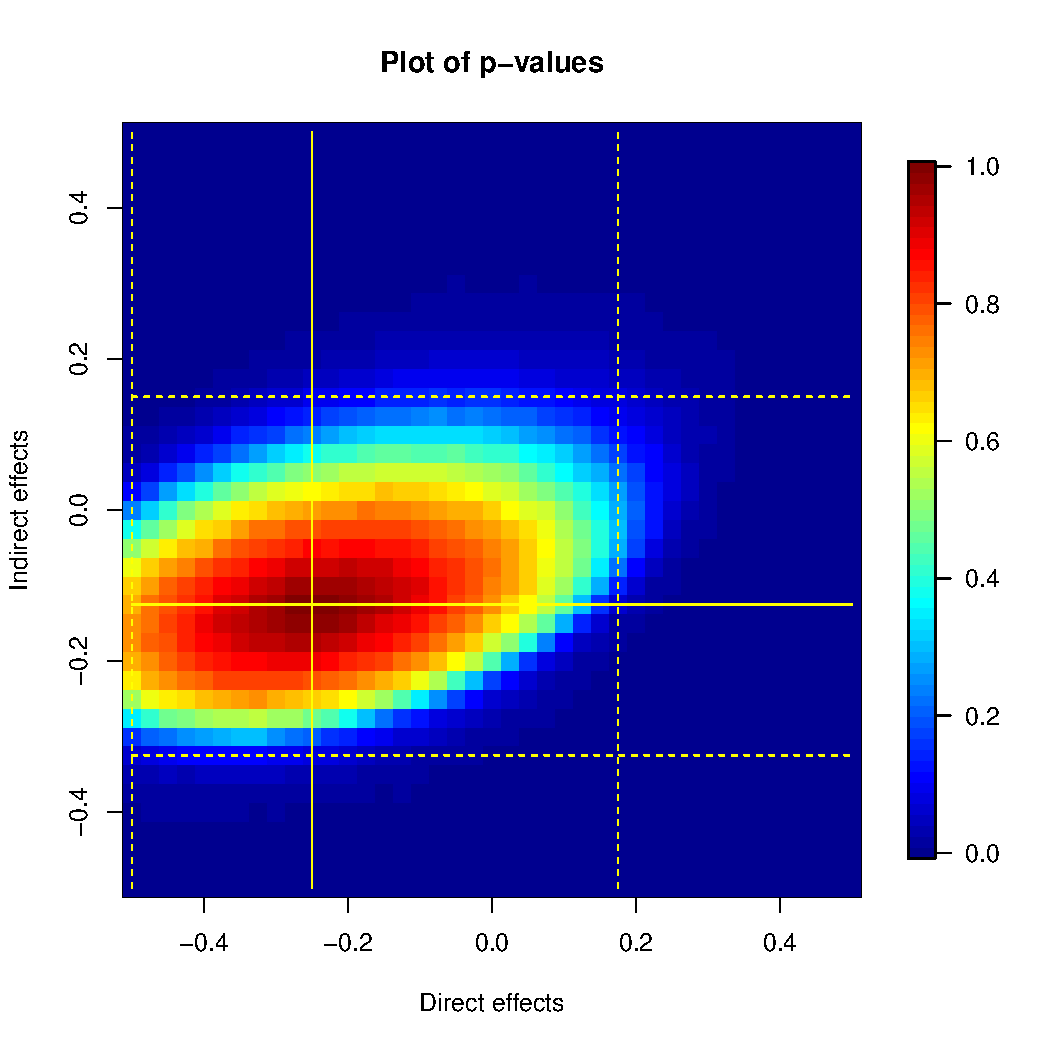
\includegraphics[scale=0.45]{./images/pval_plot_coppock_replication.pdf}
	\end{tabular}
	\caption{Main analysis for \citet{butler2011can} data}
\end{figure}


The first extension we consider is a change in the neighborhood specification. Instead of looking at ideological similarity across the network,  we consider only the nearest k neighbors at values k = 3,5,8,12.  In Figure 2, we see that the direct and indirect effects which maximize the p-value, are lower (in absolute value) than those in the first specification. When we model interference between all legislators in the network, we observe higher spillover than when looking at only nearest neighbors. We see that the observed indirect effect is higher, when considering a a broader neighborhood (the entire network being the broadest neighborhood we can consider).  Interestingly, we only see a result that is statistically significant, based on the 95\% confidence interval, when looking at the indirect effect with a neighborhood defined as the twelve nearest neighbors.
 

\begin{figure}
	\centering
	\begin{tabular}{cc}
	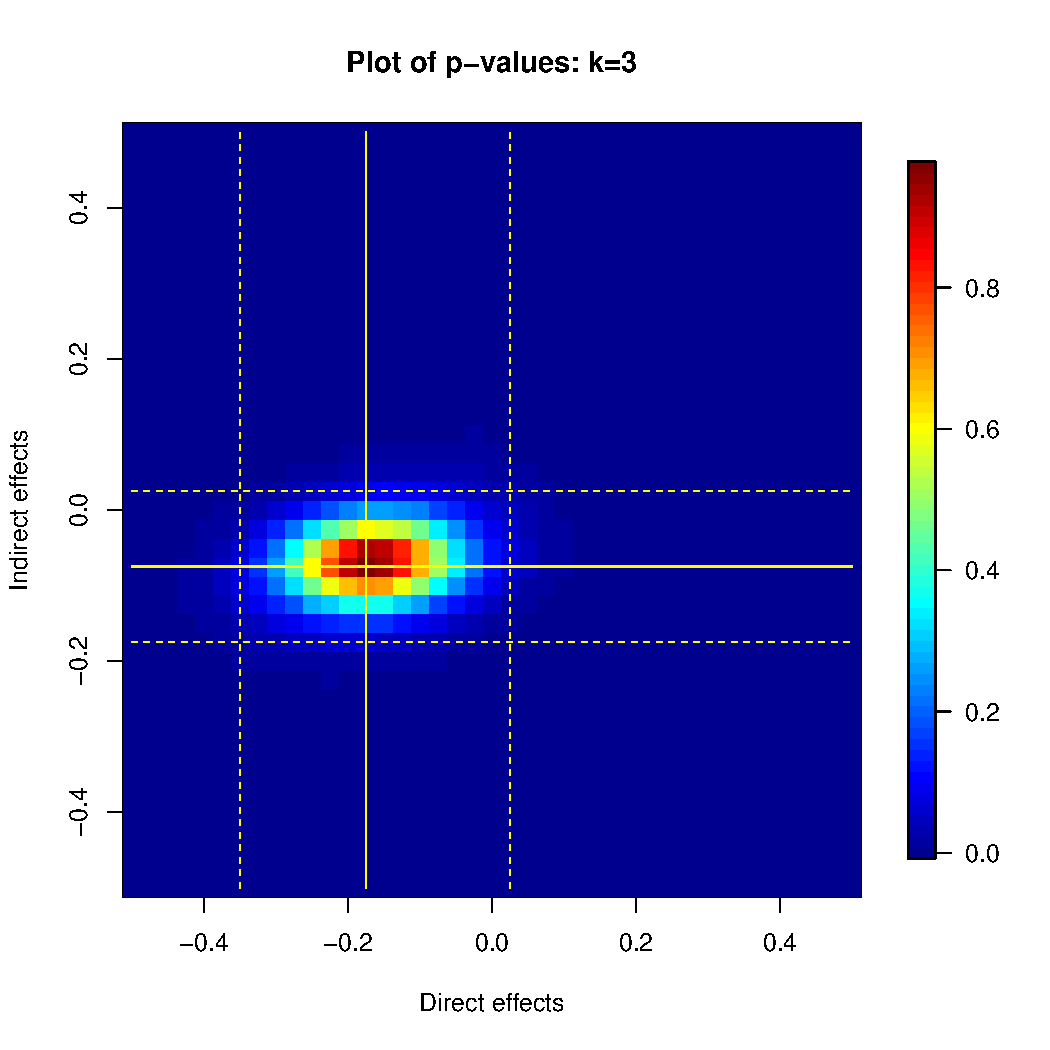
\includegraphics[scale=0.45]{./images/pval_plot_coppock_ideo_3nn.pdf} &
	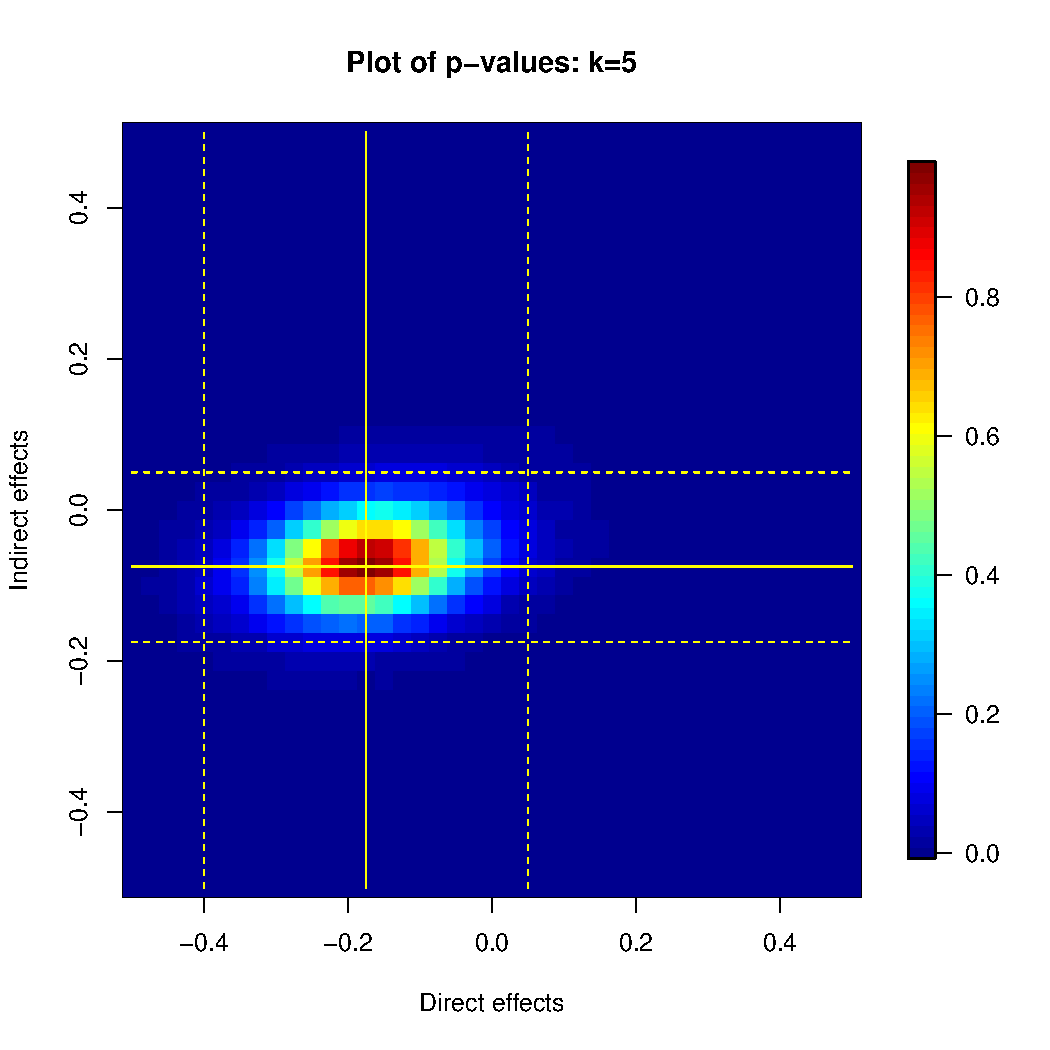
\includegraphics[scale=0.45]{./images/pval_plot_coppock_ideo_5nn.pdf} \\ 
	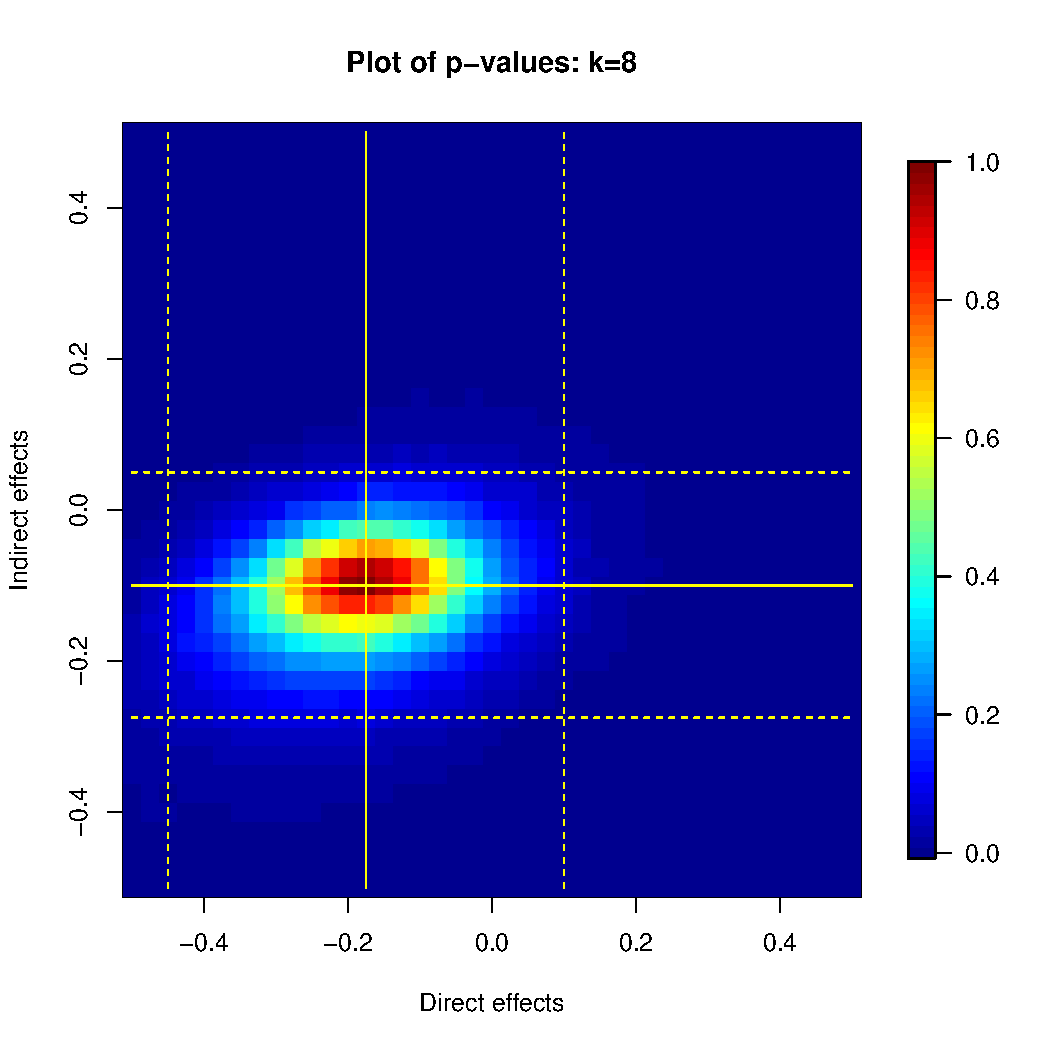
\includegraphics[scale=0.45]{./images/pval_plot_coppock_ideo_8nn.pdf} &
	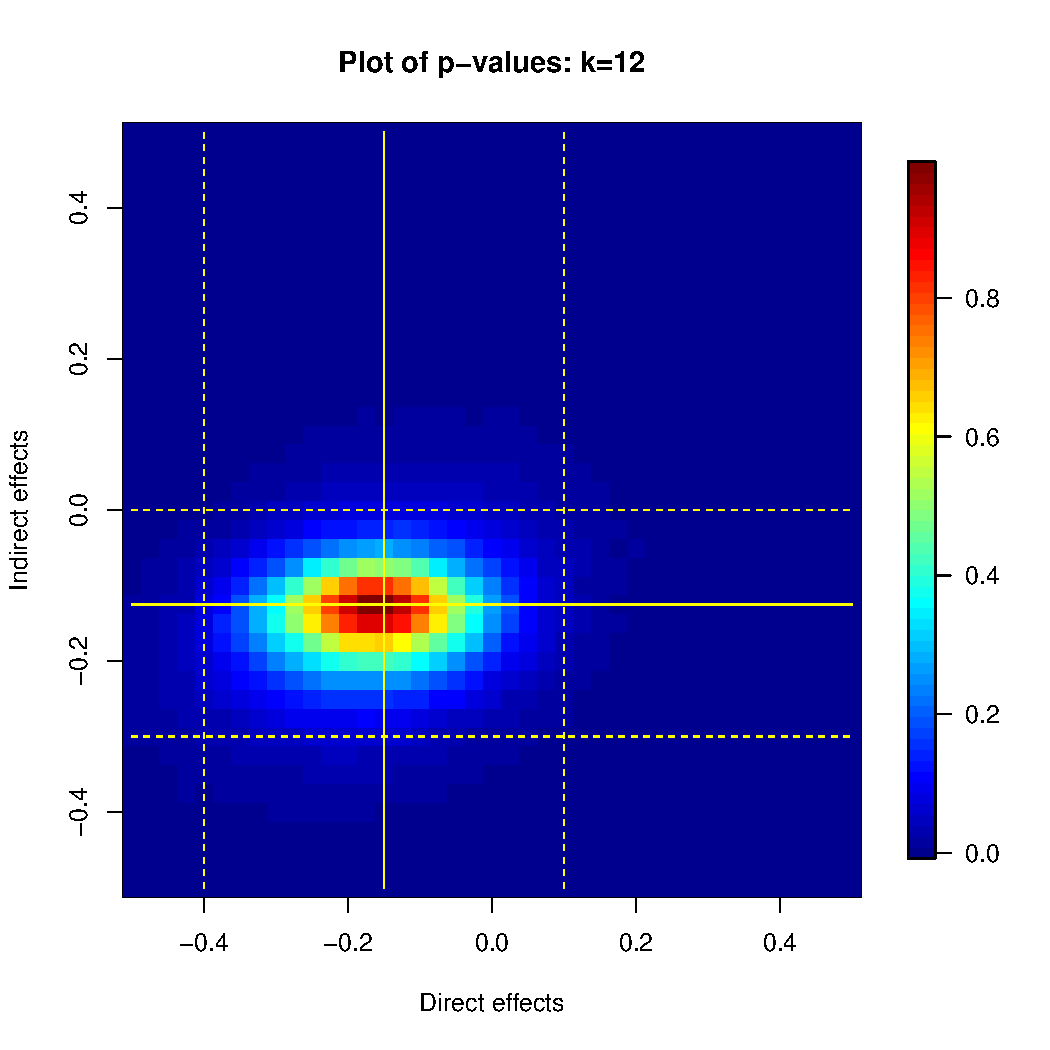
\includegraphics[scale=0.45]{./images/pval_plot_coppock_ideo_12nn.pdf} \\ 
	\end{tabular}
	\caption{k-nearest ideological neighbors for \citet{butler2011can} data}
\end{figure}


In the next extension, we change the network itself, by considering committee network. Here, an undirected edge exists between legislators who served on standing committees together.  We define the network at two thresholds---serving on at least one committee together and serving on at least two committees together. Results indicate that the committee network does not carry the effect of treatment to control units.

\begin{figure}
	\centering
	\begin{tabular}{cc}
	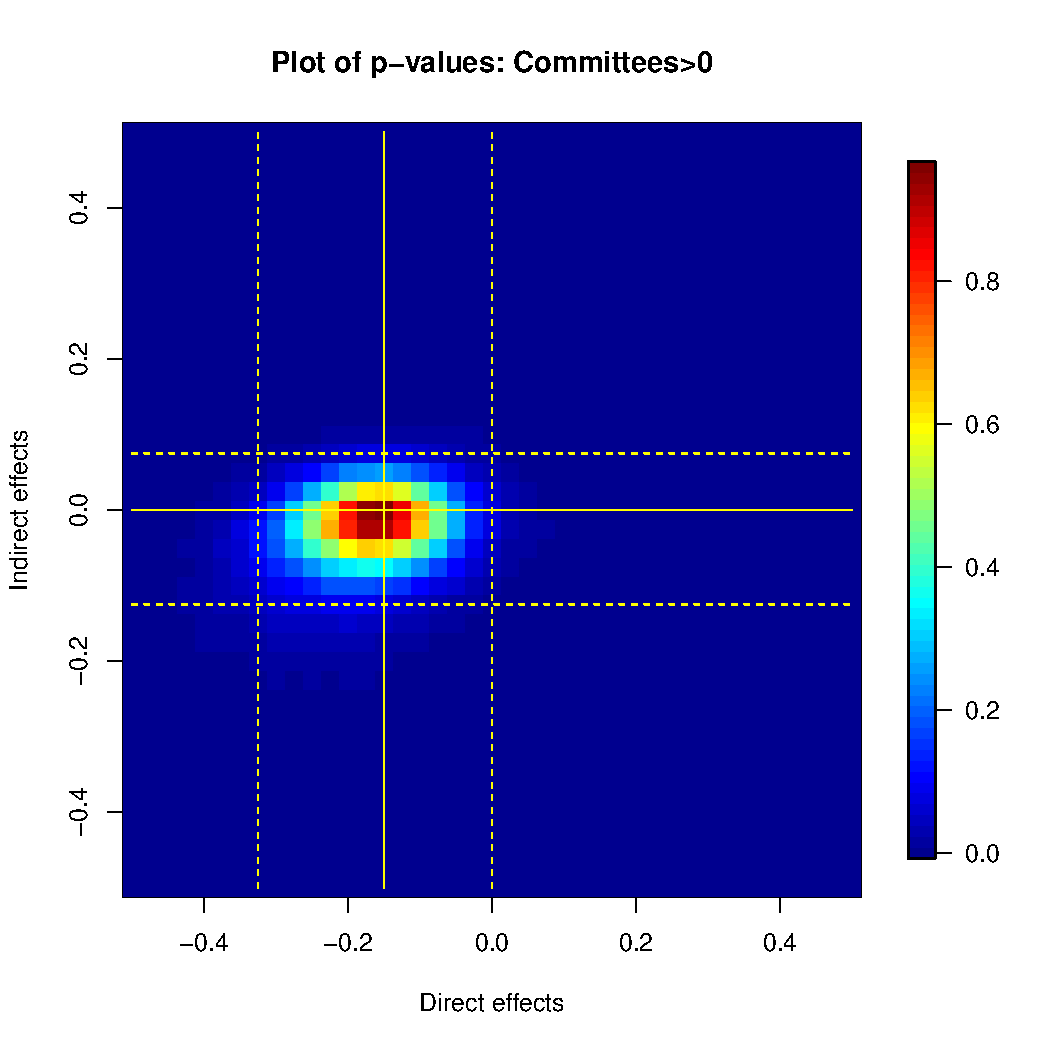
\includegraphics[scale=0.45]{./images/pval_plot_coppock_committee_1ormore.pdf} &
	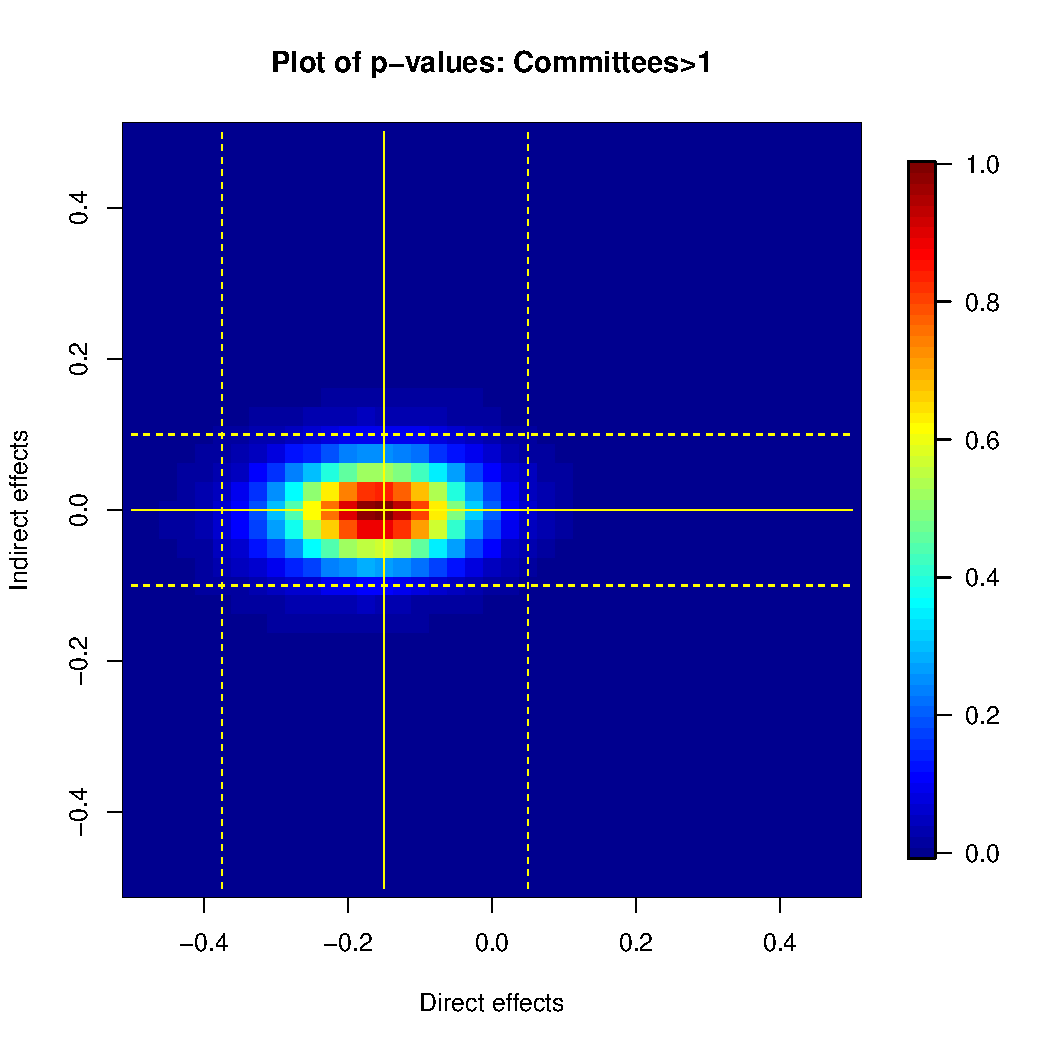
\includegraphics[scale=0.45]{./images/pval_plot_coppock_committee_2ormore.pdf}
	\end{tabular}
	\caption{Committee network for  \citet{butler2011can} data}
\end{figure}


Table 1 summarizes the results for analyzing the \citet{butler2011can} data under various specifications.  We notice that the indirect effect is negative when we consider  the  ideological  network  and  zero  when  looking  at  the  committee  network.   This emphasizes the importance of choosing a network that can best explain the phenomenon. Given that tax rebate is a fairly partisan topic,  ideological similarity can explain information spillover better than mere membership on the same committees, which is likely to be more related to seniority and non-ideological consistency composition.  We see below that the point estimate of the indirect effect is negative in all analyses that considers the ideological network, implying that as expected exposure to the treatment increases, the likelihood of a legislator to vote in favor of the tax rebate decreases.  In case of the committee network, we see that the treatment only has an effect on those who receive it directly.

\floatsetup[table]{objectset=centering,capposition=top}
\begin{table}[h]
\centering
\begin{tabular}{lcccc}
\toprule
\multirow{2}{*}{Model} & \multicolumn{2}{c}{Direct effect} & \multicolumn{2}{c}{Indirect effect} \\
\cmidrule(l){2-3} \cmidrule(l){4-5}
 & Estimate & 95\% CI & Estimate & 95\% CI \\
\midrule
Ideology: full network  & -0.25 & (-0.5, 0.175) & -0.15 & (-0.325, 0.15)\\
Ideology: 3nn & -0.175 & (-0.35, 0.025) & -0.075 & (-0.175, 0.025)\\
Ideology: 5nn & -0.175 & (-0.4, 0.05) & -0.075 & (-0.175, 0.05)\\
Ideology: 8nn & -0.175 & (-0.45, 0.10) & -0.10 & (-0.275, 0.05)\\
Ideology: 12nn & -0.15 &(-0.4,  0.1) & -0.125 & (-0.3, 0)\\
Committee: >0& -0.15 & (-0.325, 0) & 0 & (-0.125, 0.075)\\
Committee: >1 & -0.15 & (-0.375, 0.05) & 0 & (-0.1, 0.1)\\
\bottomrule
\end{tabular}
\caption{Results from \citet{coppock2014information} data}
\end{table}


% Same table as above with raw/unadjusted/unstandardized effects
%\floatsetup[table]{objectset=centering,capposition=top}
%\begin{table}[h]
%\centering
%\begin{tabular}{lcccc}
%\toprule
%\multirow{2}{*}{Model} & \multicolumn{2}{c}{Direct effect} & \multicolumn{2}{c}{Indirect effect} \\
%\cmidrule(l){2-3} \cmidrule(l){4-5}
% & Estimate & 95\% CI & Estimate & 95\% CI \\
%\midrule
%Ideology: full network  & -0.175 & (-0.35, -0.025) & -0.075 & (-0.5, 0.5)\\
%Ideology: 3nn & -0.175 & (-0.35, 0.025) & -0.05 & (-0.175, 0.025)\\
%Ideology: 5nn & -0.175 & (-0.4, 0.025) & -0.075 & (-0.2, 0.025)\\
%Ideology: 8nn & -0.175 & (-0.45, 0.1) & -0.075 & (-0.325, 0.05)\\
%Ideology: 12nn & -0.2 &(-0.45,  0.05) & -0.15 & (-0.375, -0.025)\\
%Committee: >0& -0.15 & (-0.3, 0) & -0.025 & (-0.275, 0.3)\\
%Committee: >1 & -0.15 & (-0.03, 0) & -0.025 & (-0.2, 0.15)\\
%\bottomrule
%\end{tabular}
%\caption{Results from \citet{coppock2014information} data: Raw exposure for all analysis except Full Ideological Network}
%\end{table}


\subsection{Results for \citet{bergan2015call} data}

This data has not been analyzed for indirect effects before. However, for all the reasons that we would expect to see interference in the \citet{butler2011can} results, we would expect to see them in the \citet{bergan2015call} results. We conduct an analysis similar to that in \citet{coppock2014information}, where a network is constructed based on ideological scores of legislators, using roll call data. We do not find evidence of indirect effects via this network. It is possible that we can attribute this to the nature of the bill.  Voting behavior on an anti-bullying bill may not be governed by ideological coalitions. In the next iteration of this paper we plan to consider other networks such as the standing committee network. Figure 4 shows the plot of p-values for this analysis.

\begin{figure}
	\centering
	\begin{tabular}{cc}
	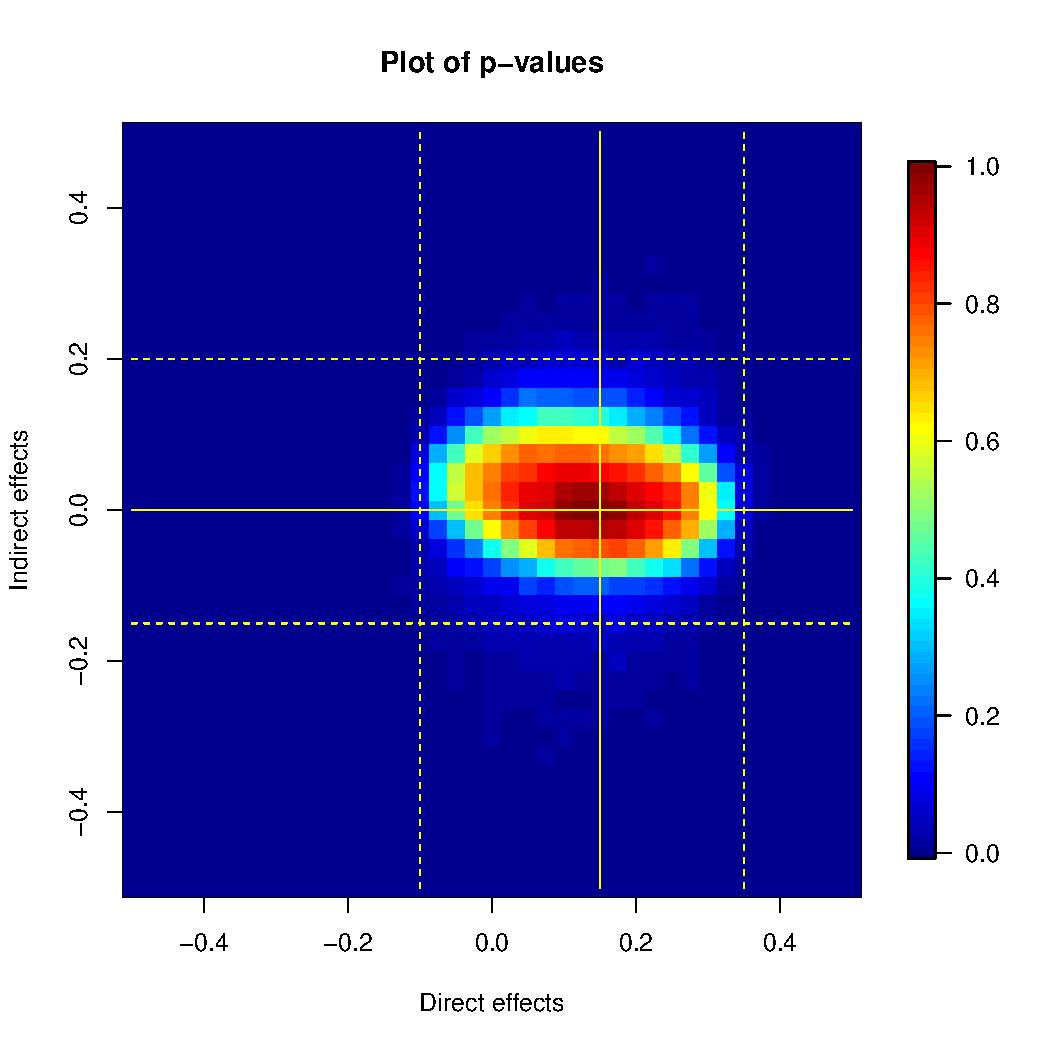
\includegraphics[scale=0.45]{./images/pval_plot_bergan_main.pdf}
	\end{tabular}
	\caption{p-values: main analysis for \citet{bergan2015call} data}
\end{figure}


Figure 5 depicts results of analyzing the \citet{bergan2015call} data under the ideological network and considers k nearest neighbors (k = 3,5,8,12) based on ideological similarity to constitute the neighborhood. We see that the results regarding indirect effects do not change and the estimate is still zero, indicating no interference effect.

\begin{figure}
	\centering
	\begin{tabular}{cc}
	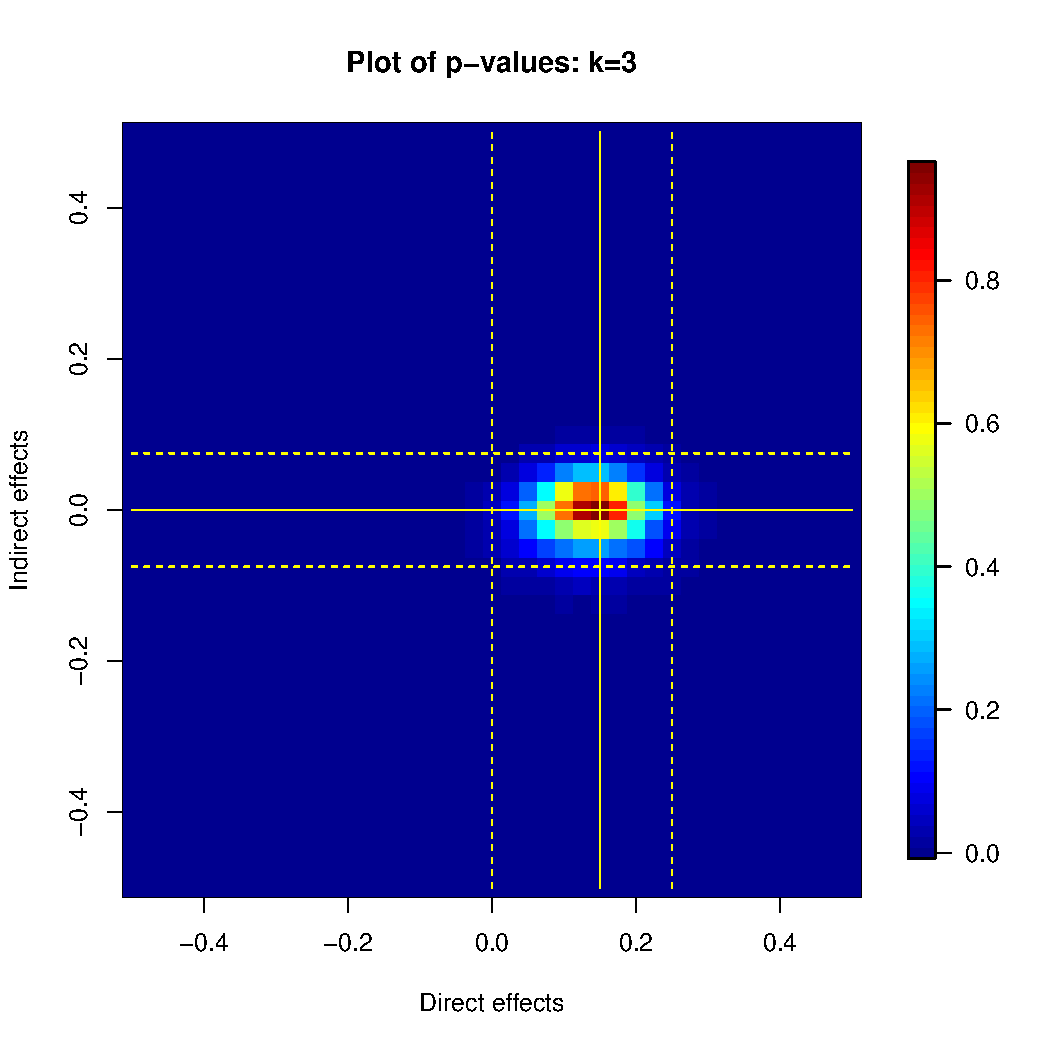
\includegraphics[scale=0.45]{./images/pval_plot_bergan_ideo_3nn.pdf} &
	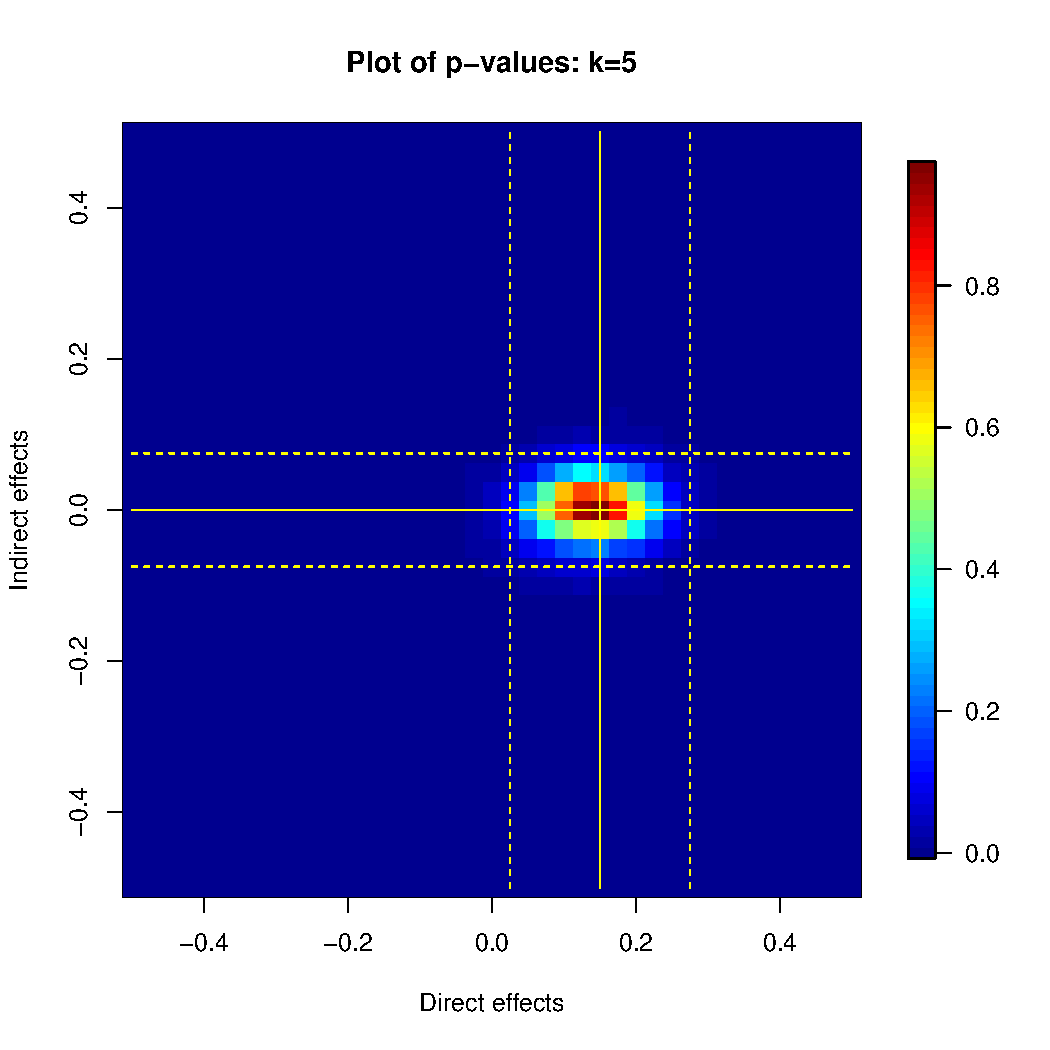
\includegraphics[scale=0.45]{./images/pval_plot_bergan_ideo_5nn.pdf} \\ 
	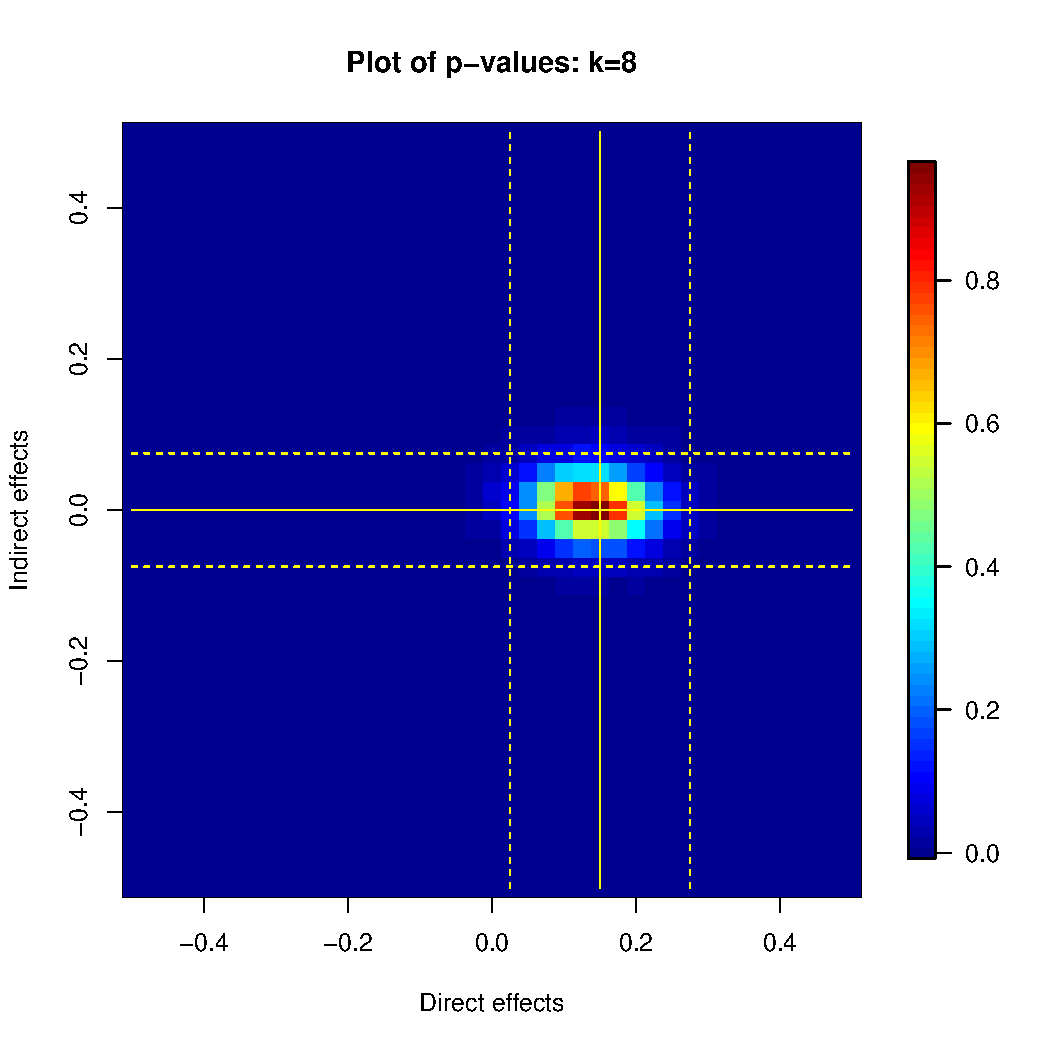
\includegraphics[scale=0.45]{./images/pval_plot_bergan_ideo_8nn.pdf} &
	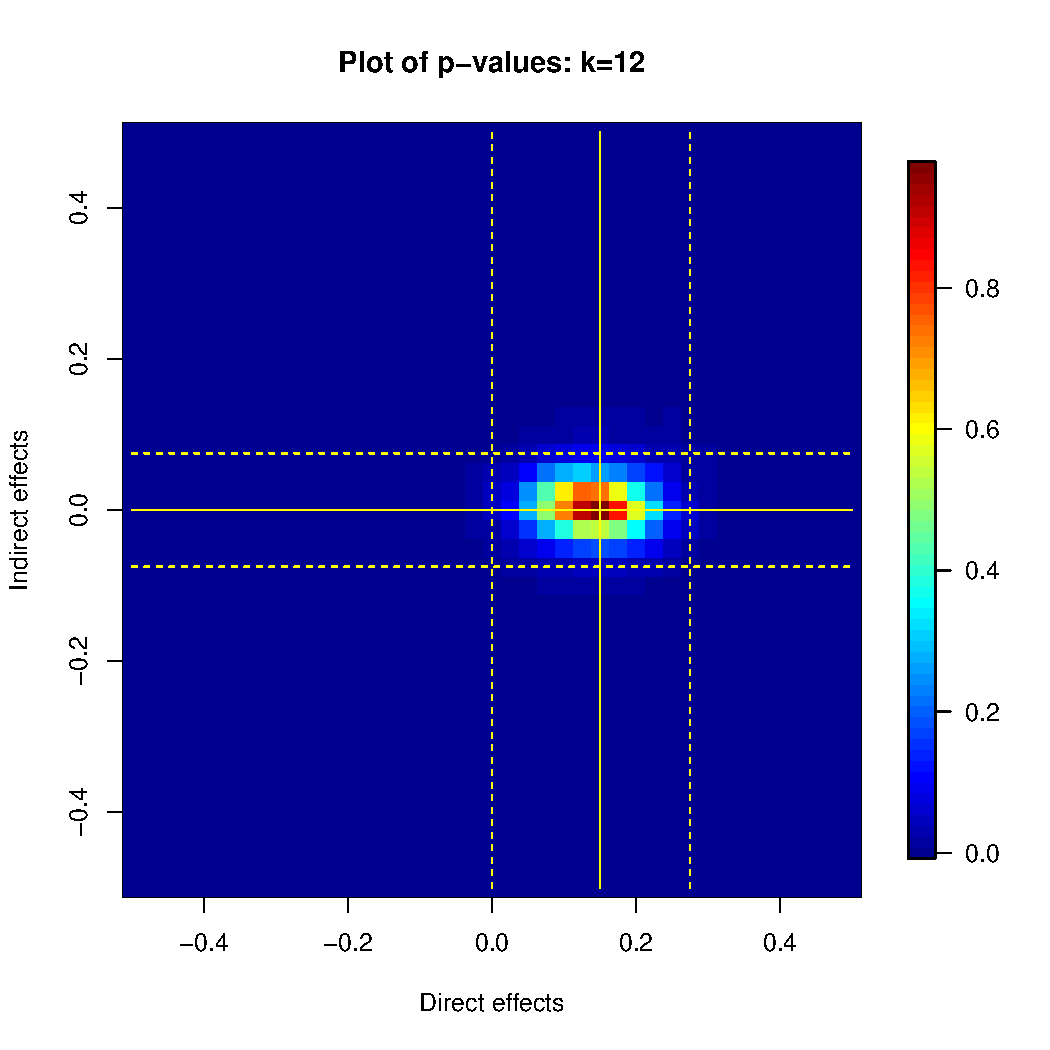
\includegraphics[scale=0.45]{./images/pval_plot_bergan_ideo_12nn.pdf} \\ 
	\end{tabular}
	\caption{p-values: k-nearest ideological neighbors for \citet{bergan2015call} data}
\end{figure}


We look at another extension where the cosponsorship network is considered. In this network, an undirected edge represents the number of bills cosponsored by a pair of legislators. We see that ties formed by cosponsoring bills carry the effect of treatment to control units. The positive indirect effect indicates that as exposure through cosponsoring neighbors goes up, the likelihood of a legislator voting in favor of the anti-bullying bill goes up. However, the confidence interval going into negative values indicates that this effect is not significant.

\begin{figure}
	\centering
	\begin{tabular}{cc}
	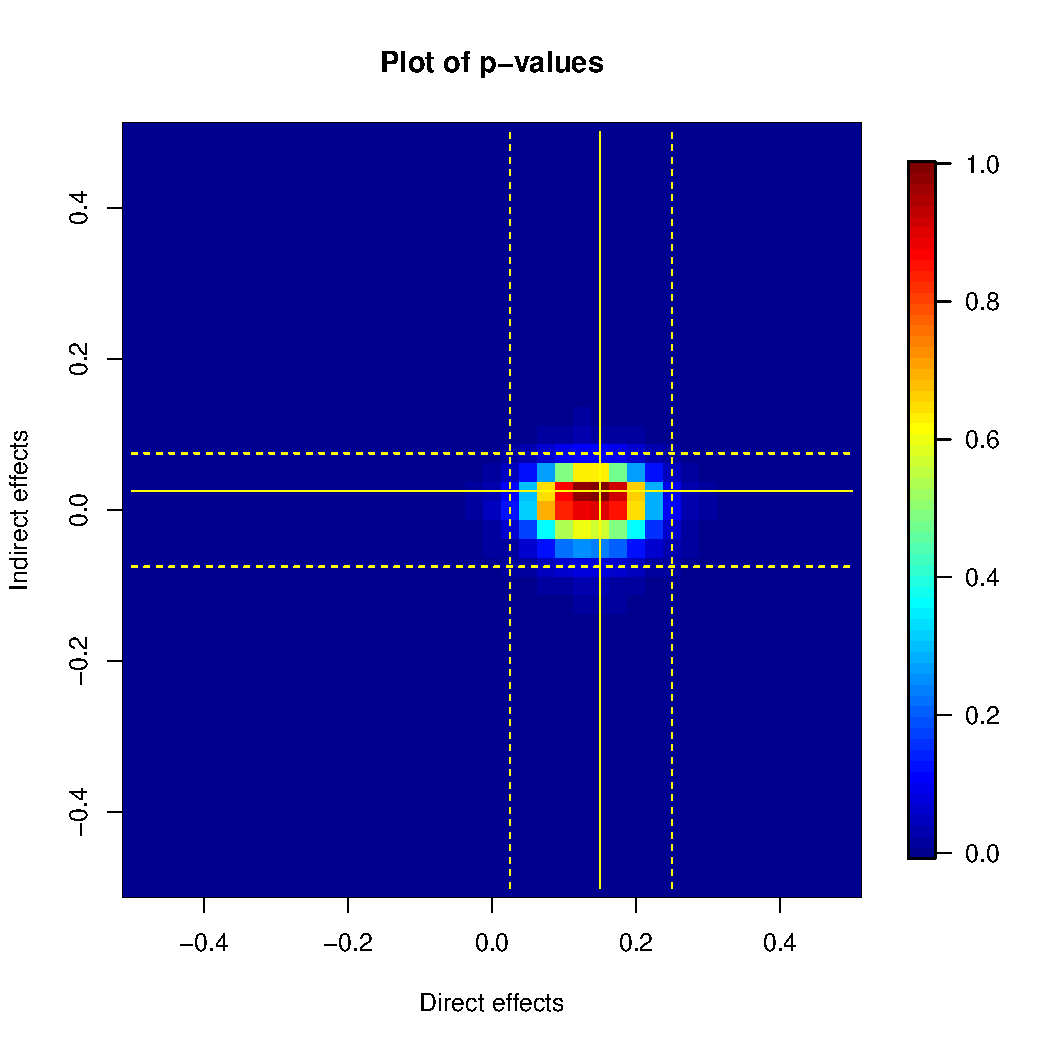
\includegraphics[scale=0.45]{./images/pval_plot_bergan_cospon.pdf}
	\end{tabular}
	\caption{p-values: Cosponsorship network for \citet{bergan2015call} data}
\end{figure}


Table 2 summarizes results of the \citet{bergan2015call}.  The point estimates are consistent across neighborhood specifications under the ideological network.


\floatsetup[table]{objectset=centering,capposition=top}
\begin{table}[h]
\centering
\begin{tabular}{lcccc}
\toprule
\multirow{2}{*}{Model} & \multicolumn{2}{c}{Direct effect} & \multicolumn{2}{c}{Indirect effect} \\
\cmidrule(l){2-3} \cmidrule(l){4-5}
 & Estimate & 95\% CI & Estimate & 95\% CI \\
\midrule
Ideology: full network  & 0.15 & (-0.1, 0.35) &  0 & (-0.15, 0.2)\\
Ideology: 3nn & 0.15 & (0, 0.25) & 0 & (-0.075, 0.075)\\
Ideology: 5nn & 0.15 & (0.025, 0.75) & 0 & (-0.075, 0.075)\\
Ideology: 8nn & 0.15 & (0.025, 0.75) & 0 & (-0.075, 0.075)\\
Ideology: 12nn & 0.15 & (0, 0.275) & 0 & (-0.075, 0.075)\\
Cosponsorship & 0.15 & (0.025, 0.25) & 0.025 & (-0.075, 0.075)\\
\bottomrule
\end{tabular}
\caption{Results from \citet{bergan2015call} data}
\end{table}


%\floatsetup[table]{objectset=centering,capposition=top}
%\begin{table}[h]
%\centering
%\begin{tabular}{lcccc}
%\toprule
%\multirow{2}{*}{Model} & \multicolumn{2}{c}{Direct effect} & \multicolumn{2}{c}{Indirect effect} \\
%\cmidrule(l){2-3} \cmidrule(l){4-5}
% & Estimate & 95\% CI & Estimate & 95\% CI \\
%\midrule
%Ideology: full network  & 0.125 & (0.025, 0.2) &  -0.05 & (-0.45, 0.5)\\
%Ideology: 3nn & 0.1 & (0, 0.2) & -0.05 & (-0.25, 0.05)\\
%Ideology: 5nn & 0.1 & (0, 0.2) & -0.05 & (-0.175, 0.05)\\
%Ideology: 8nn & 0.125 & (0, 0.225) & -0.025 & (-0.1, 0.05)\\
%Ideology: 12nn & 0.125 & (0, 0.225) & 0 & (-0.075, 0.075)\\
%Cosponsorship & 0.125 & (0.025, 0.2) & 0.075 & (-0.5, 0.5)\\
%\bottomrule
%\end{tabular}
%\caption{Results from \citet{bergan2015call} data: Raw exposure}
%\end{table}


\subsection{Results for \citet{broockman2013black} data}

We now discuss the last application considered in this paper. As discussed in the earlier section, the author of this paper analyzed the data assuming SUTVA. However, it would be reasonable to expect that legislators within each state communicate with each other leading to spillover of treatment effect. We stipulate three possible networks through which interference may occur. These depend on two key covariates; Percentage of Democratic Vote ($demvotepercent$) in the district, and Percentage of Black Legislators ($blackpercent$) in the district. We create one network for each of the two covariates and a third combining the two. In networks based on individual variables, similarity score for legislators $i$ and $j$ based on variable $X$ is defined as in Equation (1).

\begin{equation}
Similarity_{(i,j)} = \frac{2 - |x_i - x_j|}{2}
\end{equation}

For the network based on two covariates, network is defined as the Euclidean distance between legislators $i$ and $j$ where $demvotepercent$ ($X$) and $blackpercent$ ($Y$) are equally weighted, as shown in Equation (2).

\begin{equation}
Similarity_{(i,j)} = \sqrt{{(x_i - x_j)}^2 + {(y_i - y_j)}^2}
\end{equation}

In these block-diagonal networks, neighborhood of any legislator consists of all other legislators in his/her state. The closer any two units are on values of one of these variables, the stronger the tie, and higher the exposure to receiving indirect treatment. Figures 6 and 7 depict results of analyzing the \citet{broockman2013black} data under the combined network and the individual networks respectively. We see that two of these three specifications show evidence of spillover effect.


\begin{figure}
	\centering
	\begin{tabular}{cc}
	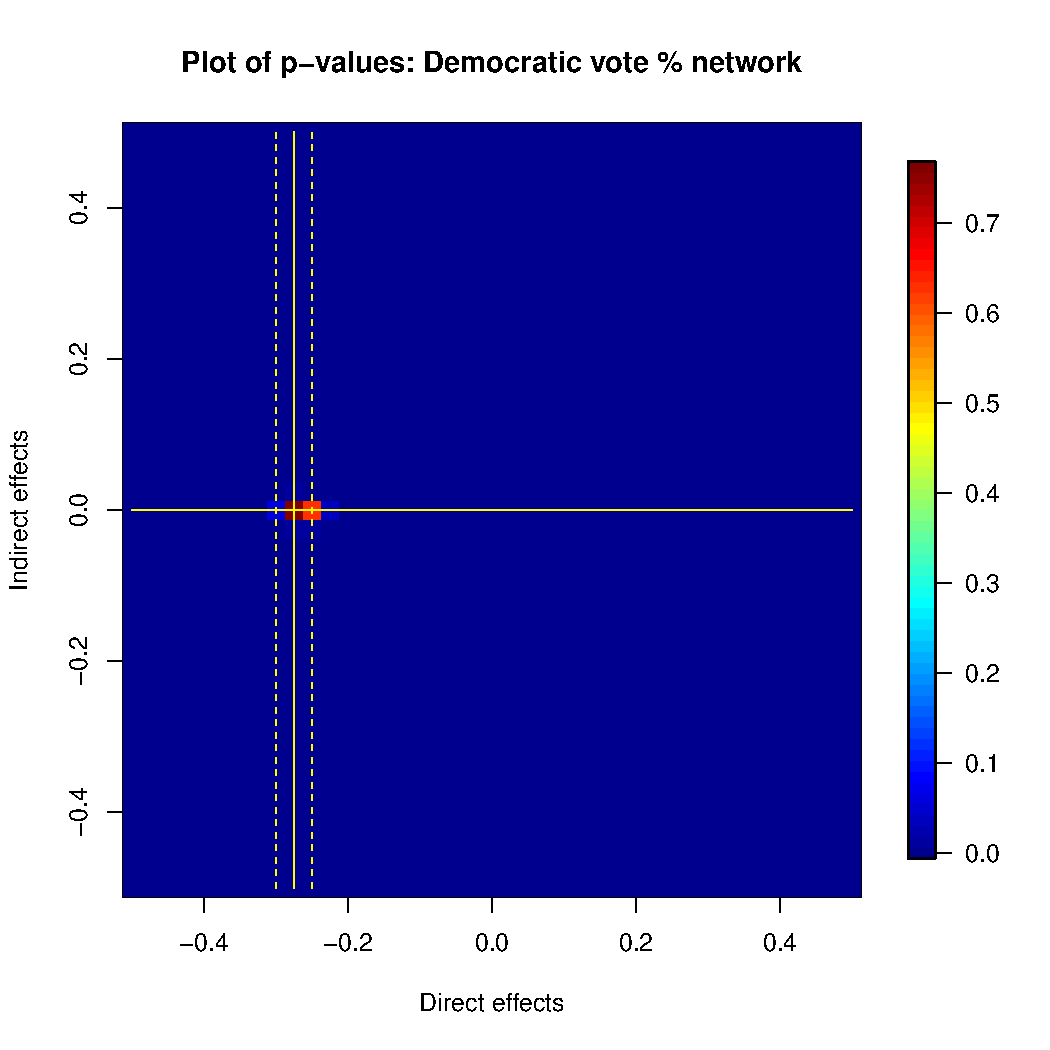
\includegraphics[scale=0.45]{./images/pval_plot_broockman_demvotepct.pdf} &
	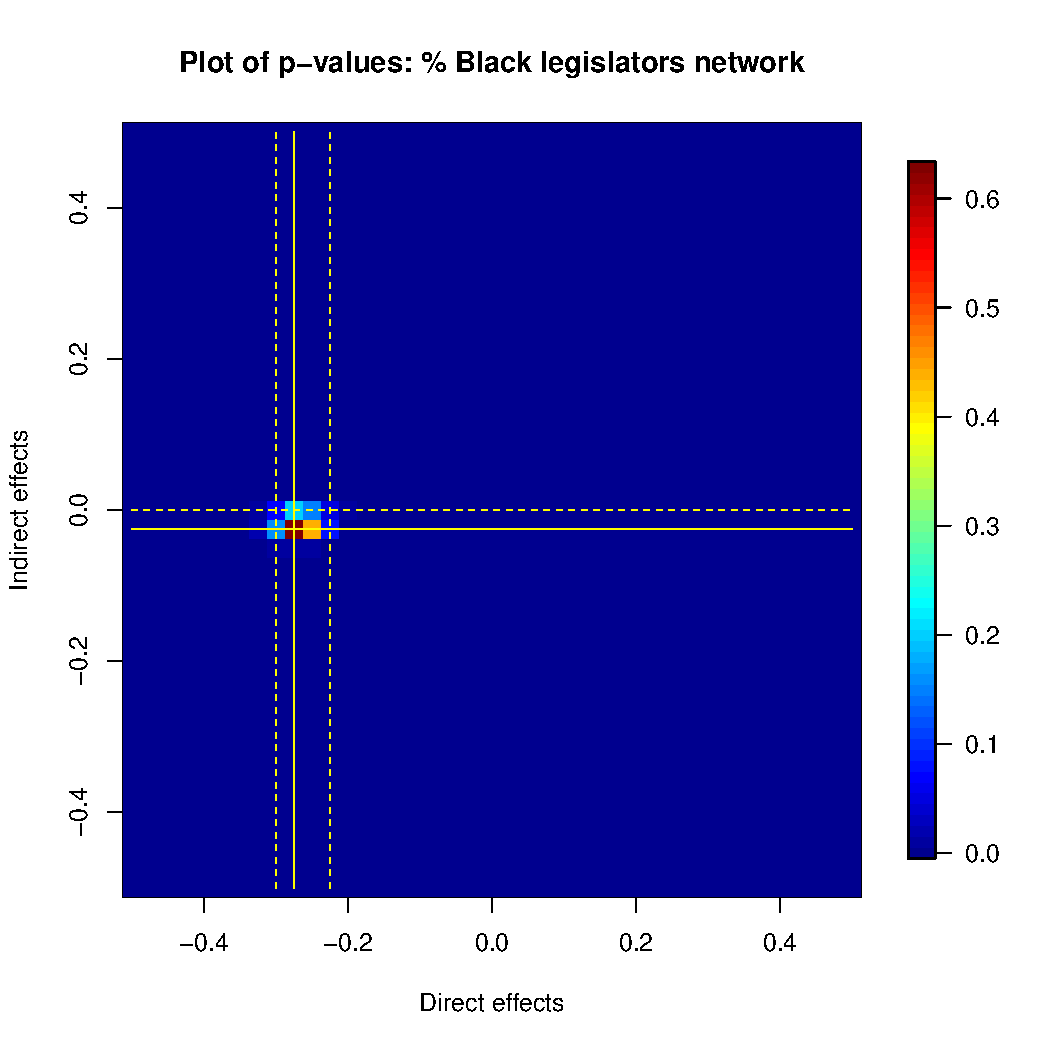
\includegraphics[scale=0.45]{./images/pval_plot_broockman_blackpct.pdf} \\ 
	\end{tabular}
	\caption{p-values for \citet{broockman2013black} data}
\end{figure}

\begin{figure}
\centering
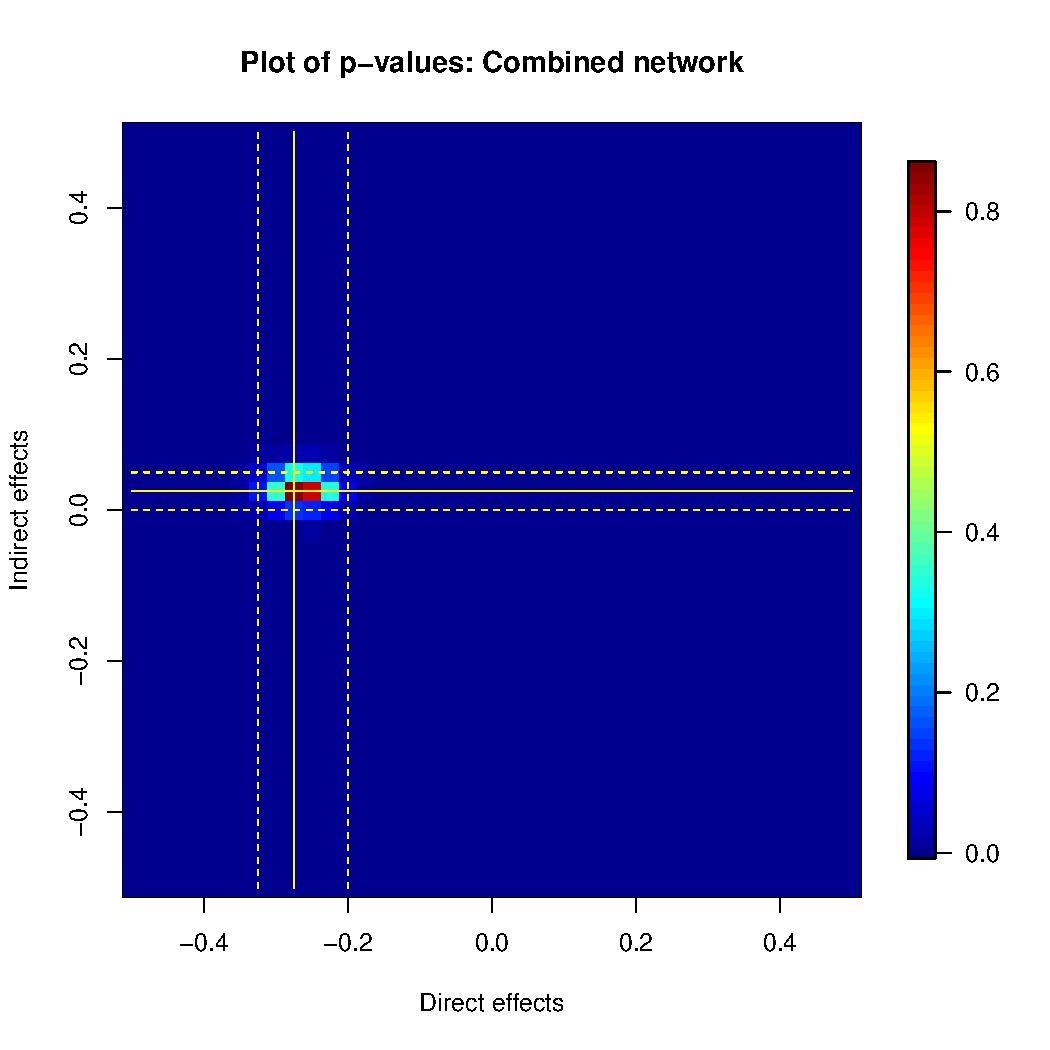
\includegraphics[scale=0.45]{./images/pval_plot_broockman_demvotepct_blackpct.pdf}
\caption{p-values for \citet{broockman2013black} data: Combined network}
\end{figure}


This is further detailed in table 5. The non-zero point estimates indicate spillover of treatment to control units. It is interesting to note though, that these values have different signs for the $blackpercent$ and the combined network. When exposure is via legislators with similar values of $blackpercent$, the likelihood of the legislator to respond to Tyrone reduces. In contrast, as exposure through the combined network increases, the likelihood of responding to Tyrone increases. Each of these confidence intervals crosses over zero, therefore the effects are not significant. The setup of the similarity score is such, that for a given state, the number of legislators with either high or low $demvotepercent$ and $blackpercent$ can dominate the overall effect.


\floatsetup[table]{objectset=centering,capposition=top}
\begin{table}[h]
\centering
\begin{tabular}{lcccc}
\toprule
\multirow{2}{*}{Model} & \multicolumn{2}{c}{Direct effect} & \multicolumn{2}{c}{Indirect effect} \\
\cmidrule(l){2-3} \cmidrule(l){4-5}
 & Estimate & 95\% CI & Estimate & 95\% CI \\
\midrule
Democratic vote percentage & -0.275 & (-0.3, -0.25) &  0 & (0, 0)\\
Percentage of black legislators & -0.275 & (-0.3, -0.225) &  -0.025 & (-0.025, 0)\\
Mixture network & -0.275 & (-0.325, -0.2) &  0.025 & (0, 0.05)\\
\bottomrule
\end{tabular}
\caption{Results from \citet{broockman2013black} data}
\end{table}


%\subsection{Extensions of Coppock analysis}
%We consider several extensions of the Coppock method, applied to both datasets depending on availability of data.
%
%\begin{itemize}
%\item Consider k (=3, 5, 8, 12) neighbors according to ideological scores to form adjacency matrix. A tie between i and j indicates that legislator j is one of the k-nearest neighbors to i. This generates some ties. We will try the following two ways of taking care of the ties:
%
%\begin{enumerate}
%\item Choose, among the ties in the k closest neighbors for i, those nodes for which i is the closest neighbor. To illustrate, if i is equally close to j and h, we ask whether i ranks higher on j's list of closest neighbors. If yes, then we take out h. If no, we keep j and h if i ranks equally on j and h's neighbor list, or kick out j if h ranks i more highly.
%\item Look at the number of nodes for which j is the nearest neighbor and in some way account for the j's influence on that basis
%1. Look at control unit i
%2. Calculate a composite score that indicates the ranking of i for each of its k neighbors
%3. Estimate a parameter to see if change in composite score leads to a change in propensity for changing the outcome
%4. This parameter will be modeled as a non-linear effect
%For example, say k=3 condition. If a control unit is the lowest in the proximity of all of its 3 neighbors, it is less likely to receive a spillover; as compared to if it was in the highest proximity of all three of them (the two extremes). We would have to condition this on the treatment status of its neighbors.
%\end{enumerate}
%
%\item Consider committee network instead of ideological network, where a tie between i and j indicates that they have served on two or more committees together
%\item Use number of shared committees in adjacency matrix
%\item Separate out the high and low support district in original \citet{butler2011can} data and conduct separate analyses. This would explain the direction of the spillover effect much better. Conduct this analysis with ideological network as well as committee network
%\item Include geographical network in both dataset and extend analysis
%\item Consider various spillover models other than the growth curve specification
%\item Consider weighted combinations of different networks to estimate a $\gamma$
%\item Explore the idea of using communities to model spread across the network
%
%\end{itemize}

\section{Discussion}
The results from our replication of field experiments on legislatures underscore the importance and complexity of accounting for interference in field experiments on interactive groups. The replications and extensions of \citet{coppock2014information} and \citet{bergan2015call} demonstrate both the presence of interference effects, and the inferential consequences of choices in specifying both the network and the neighborhood through which treatment is hypothesized to propagate. These two applications are focused on roll call votes as the outcomes. These are important legislative actions, but may be constrained in terms of their susceptibility to experimental manipulations in that they are heavily centralized and subject to open and widespread scrutiny. The \citet{broockman2013black} study, in contrast, considers the effects of the manipulation on responses to individualized requests---requests that were initialized as part of the experiment. Results from this analysis emphasize the importance of thinking about not only the possible network, but also the resulting interpretation of the indirect effect parameter. The replication and extension of \citet{bergan2015call} illustrates that interference effects will not be evident in every field experiment, even in network types that were found to propagate treatment in other studies. 


In the next iteration of this paper, we plan to extend the analysis in three directions. First, we will gather additional network data to use in testing for interference in---at the very least---the \citet{bergan2015call} replication. \textcolor{red}{I don't remember why we emphasized on Bergan. Maybe because the indirect effects were zero when looking at expected exposure?} One important caveat regarding our replications is that we do not have access to the multitude of relational data that scholars have used to define legislative networks. We will make an effort to gather additional legislative network data to use in our replications. Second, we have not yet considered the count vs balance dimension in the specification of the interference models in our replication. Incorporating this dimension will allow us to compare models in which connections to control units counteract the effects to treated units, as compared to the current results, which attribute interference solely to the number of of treated units in a node's neighborhood. \textcolor{red}{In the earlier draft, Broockman analysis was the third proposed change. However, that is now a part of the main paper. So we can select something from the first section. Maybe we look at a different outcome variable, or a different test statistic?}

%%%%
\section{Conclusion}
%%%%


% What we have demonstrated
We make the case that many common domains in which political scientists employ field experiments present conditions under which we would expect interference, which represents a violation of SUTVA. These domains concern experiments on interactive social groups. We review the use of recently developed methods for testing causal models in the context of interference, and present several dimensions that researchers should consider in specifying causal models that involve interference. Through a broad replication and extension exercise focused on field experiments on legislatures, we illustrate consideration of these dimensions and show that evidence for interference exists, and depends upon the choices made in specifying the causal models.


% Implications for future research
Our arguments and results lead to three important implications in future research. First, when analyzing results from field experiments that target populations within which there is a risk of interaction, and therefore interference, researchers must consider the consequences of interference for their inferences. Second, our results underscore the opportunities for researchers to develop new theoretical inquiries focused on interference. Field experiments on interactive groups have become commonplace in research designs in political science. Furthermore, we now have methods available for testing interference hypotheses. These two factors combine to open the door to principled empirical and experimental tests of interference hypotheses. Third, since the optimal experimental design depends upon the network and hypothesized model of effects \citep{bowers2016models}, researchers should incorporate considerations regarding interference before fielding their experiments. %In discussing a simulation example that revealed complex ways in which statistical power depended upon the proportion assigned to treatment, \citet[p. 113]{bowers2012reasoning} advised, ``we strongly encourage researchers to perform similar power simulations before deciding how to allocate treatment.''

%\clearpage
\bibliographystyle{apsr}
\bibliography{interference}

\end{document}
%%%%
\section{Network plots}
%%%%

\begin{figure}
\centering
\begin{tabular}{cc}
{\bf Geographic Network} & {\bf Committee Network (>1 in common)}\\
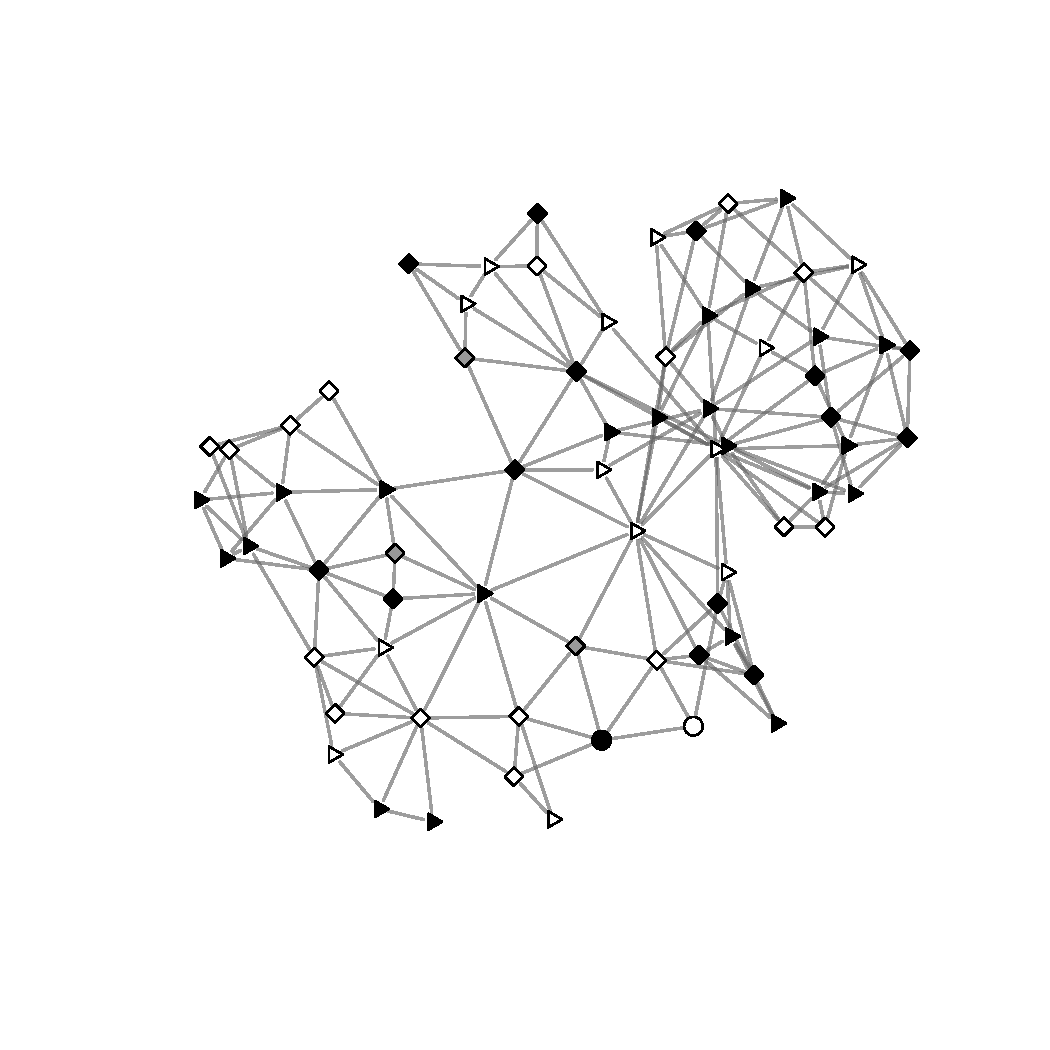
\includegraphics[scale=.55, clip=true,trim =2cm 2cm 2cm 2cm ]{./images/coppock_geographic_net.pdf} & 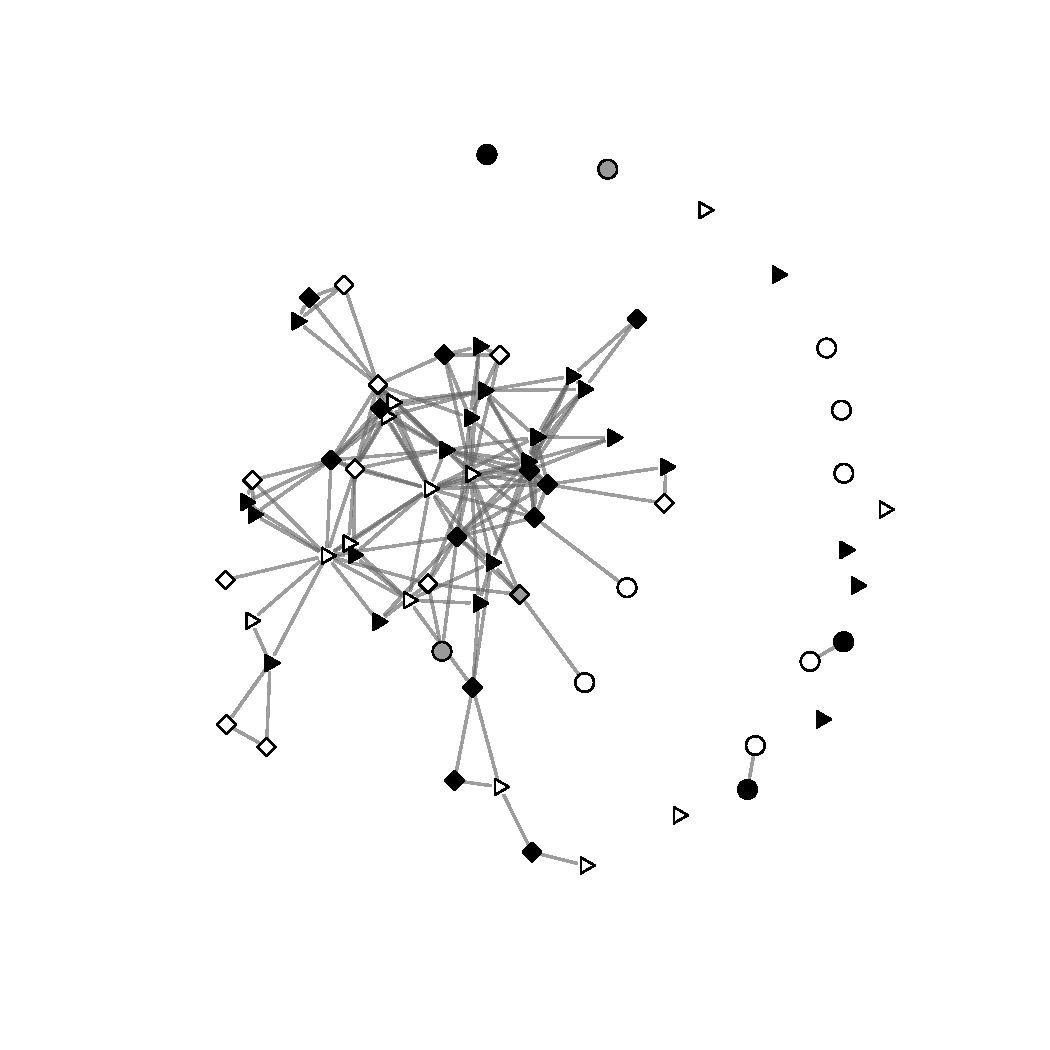
\includegraphics[scale=.55, clip=true,trim =2cm 2cm 2cm 2cm]{./images/nm_committee_net.pdf} \\ 
\end{tabular}
{\bf Ideological Network (top 5\%)} \\
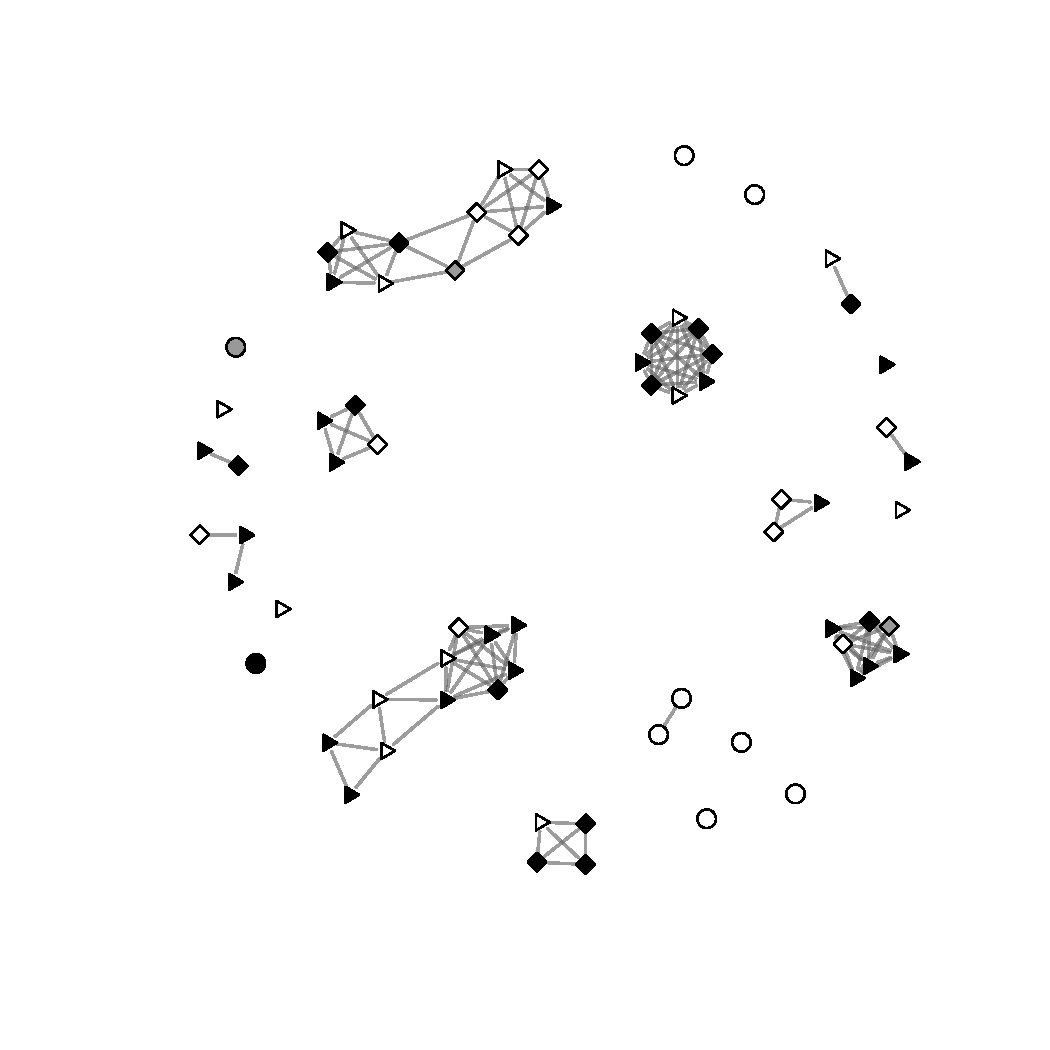
\includegraphics[scale=.55, clip=true,trim =2cm 2cm 2cm 2cm]{./images/coppock_ideological_net.pdf}
\caption{Different networks among New Mexico legislators. Colors denote outcome: black means voted with district, gray means abstained, white means voted against. Shape denotes treatment status. Triangles are treated. Squares are adjacent to treated. Circles are isolated from treatment}
\label{figure: nh-nets}
\end{figure}


%%%%
\section{Appendix}
%%%%

\subsection{Appendix 1A}

In this section, we will look at user-defined R-functions that replicate the \citet{bowers2012reasoning} methodology. This contains four steps:

\begin{itemize}
\item A function to transform the observed outcomes into potential outcomes for any treatment assignment w
\item A function to separate the hypothesized treatment effect
\item A function to calculate test statistic
\item A function to calculate the p-value.
\end{itemize}

The results from the ks.test function in R for calculating Kolmogorov-Smirnoff test statistic are verified with that in Footnote 12 of the paper.


\textbf{Function 1: calculating potential outcomes}

\begin{lstlisting}[language=R]
set.seed(132)

library(doParallel)
library(foreach)
library(kSamples)
library(network)
library(permute)

#### Potential outcomes ####

#### Transform uniformity trial outcome into observed outcome
unif.to.z <- function(z, S, y.0, beta, tau){
  # z: observed treatment assignment
  # S: adjacency matrix
  # y.0: outcome vector for uniformity trial
  # beta: growth curve parameter
  # tau: rate of growth parameter  
  scalar <- as.vector(t(z)%*%S)
  spillover <- rep(NA, n)  
  spillover <- beta + ((1-z) * (1-beta) * exp(-tau^2 * scalar))  
  # This is equation 4
  h.y0.z <- spillover*y.0
}

#### Transform observed outcome into uniformity trial outcome
z.to.unif <- function(z, S, y.z, beta, tau){
  # z: initial treatment assignment
  # S: adjacency matrix
  # y.z: observed outcome vector
  # beta: growth curve parameter
  # tau: rate of growth parameter
  scalar <- as.vector(t(z)%*%S)
  spillover <- rep(NA, n)  
  # Equation (3) from paper
  spillover <- beta + ((1-z) * (1-beta) * exp(-tau^2 * scalar))
  # Equation (5) from paper
  h.yz.0 <- (1/spillover)*y.z
}

#### Transform observed outcome into outcome for ANY other assignment w
z.to.w <- function(z, S, w, y.z, beta, tau){
  # z: initial treatment assignment
  # S: adjacency matrix
  # w: new treatment assignment
  # y.z: vector of outcomes for z
  # beta: growth curve parameter
  # tau: rate of growth parameter
  scalar.z <- as.vector(t(z)%*%S)
  scalar.w <- as.vector(t(w)%*%S)
  
  spillover.z <- rep(NA, n)
  spillover.z <- beta + ((1-z) * (1-beta) * exp(-tau^2 * scalar.z))
  
  spillover.w <- rep(NA, n)
  spillover.w <- beta + ((1-w) * (1-beta) * exp(-tau^2 * scalar.w))
  
  # Equation (6) from paper
  h.z.to.w <- (spillover.w / spillover.z) * y.z
}

#### Testing and p-value calculation ####
p.val <- function(z, y.z){
  
  cl <- makeCluster(4) #Setup for parallel computing
  registerDoParallel(cl)
    
  # Calculate the outcome vector after taking away the effect of treatment
  y.0 <- z.to.unif(z=z, S=S, y.z=y.z, beta=beta, tau=tau)
  
  # Calculate test statistic
  test.stat <- ks.test(y.0[z==1], y.0[z==0],
                       alternative = "g")$statistic
  sign <- noquote(strsplit(names(test.stat), NULL)[[1]])[3]
  if(sign=="+"){
    test.stat <- test.stat
  }else{
    test.stat <- test.stat*-1
  }  
  
  # Calculate a vector of test statistic using permutations
  results <- foreach (i = 1:perms) %dopar%{
    require(permute)
    perm.z <- z[sample(1:length(z),length(z),rep=F)]
    perm.test.stat <- ks.test(y.0[perm.z==1], y.0[perm.z==0],
                              alternative = "g")$statistic
    sign <- noquote(strsplit(names(perm.test.stat), NULL)[[1]])[3]
    
    if(sign=="+"){
      return(perm.test.stat)
    }else{
      return(perm.test.stat*-1)
    }
  }
  stopCluster(cl)
  
  # A vector of test statistics
  all.test.stat.vals <- unlist(results)
  
  # Calculating p-value
  pval <- sum(all.test.stat.vals > test.stat)/perms
  return(pval)
}
\end{lstlisting}


\subsection{Appendix 1B}

Below code replicates the \citet{coppock2014information} results using the framework setup in the Bowers replication code

\begin{lstlisting}[language=R]

set.seed(231)
library(doParallel)
library(fields)
library(foreach)
library(kSamples)
library(network)
library(permute)
library(wnominate)

permute.within.categories <- function(categories,z){
	ucategories <- unique(categories)
	perm.z <- rep(NA,length(z))
	for(c in ucategories){
		z.c <- z[which(categories==c)]
		perm.z.c <- sample(z.c,length(z.c),rep=F)
		perm.z[which(categories==c)] <- perm.z.c
	}
	perm.z
}

#### Read the original Butler and Nickerson data
data <- read.table("nm.replication.tab", sep="\t", header=TRUE)
z <- data$treatment #observed treatment
y.z <- data$sb24 #observed outcome
n <- length(y.z) #number of observations
t <- length(z[z==1]) #number of treated units
perms <- 10000 #number of permutations to use in generating expected exposure
perms.test <- 5000 #number of permutations used in testing

# Function to generate adjacency matrix using similarity scores
get.similarity <- function(x, y){
  return((2-abs(x-y))/2)
}

load("CoppockJEPS.rdata")
dwnom_scores <- CoppockJEPS$dwnom_scores

## Create an adjacency/similarity matrix using ideology
S.ideo <- matrix(NA, ncol=70, nrow=70)
for (i in 1:70){
  for (j in 1:70){
    S.ideo[i,j] <- get.similarity(dwnom_scores[i], dwnom_scores[j])
  }
}
diag(S.ideo) <- 0
S.ideo[is.na(S.ideo)==T] <- 0


#### Generate expected exposure
perm <- replicate(perms, permute.within.categories(data$match_category,z))
expected.exp0 <- rep(0, n)
expected.exp1 <- rep(0, n)
for(p in 1:ncol(perm)){
  zp <- perm[,p]
	for(i in 1:n){
		if (zp[i] == 1){
				expected.exp1[i] <- expected.exp1[i] + sum(S.ideo[i,]*zp)
			}
			else{
				expected.exp0[i] <- expected.exp0[i] + sum(S.ideo[i,]*zp)
			}
	}
}
num_treat <- apply(perm,1,sum)
num_control <- apply(1-perm,1,sum)
expected.exp1 <- expected.exp1/num_treat
expected.exp0 <- expected.exp0/num_control

#### Generate expected and net exposure
#### This is the spillover effect model
indirect.treatment <- function(permutation, adj.mat){ #any treatment assignment vector and adjacency matrix can be used
 # permutation: can be the initial treatment assignment or a permutation
 raw.exp <- rep(NA, n)
 for (i in 1:n){
   raw.exp[i] <- sum(adj.mat[i,]*permutation)
   }
 net.exp <- raw.exp - (permutation*expected.exp1 + (1-permutation)*expected.exp0)
 standard.exp <- (net.exp - mean(net.exp))/sd(net.exp) #this is the spillover or indirect effect
 return(standard.exp)
}

#### We now model the uniformity trial transformation
z.to.unif <- function(outcome, beta1, beta2, permutation, adj.mat){
  # outcome: vector of direct treatment outcomes
  # beta1: direct treatment effect parameter
  # beta2: indirect treatment effect parameter
  # permutation: vector of a permutation of z (can be z itself)
  # adj.mat: adjacency matrix
  exposure <- indirect.treatment(permutation, adj.mat)
  # This is equation 5
  h.yz.0 <- outcome - (beta1*permutation) - (beta2*exposure)
  return(h.yz.0)
}

#### Testing and p-value calculation
beta1s <- seq(from=-0.5, to=0.5, by=.025)
beta2s <- seq(from=-0.5, to=0.5, by=.025)
pvals <- matrix(NA, length(beta1s), length(beta2s))

cl <- makeCluster(8) #Setup for parallel computing
registerDoParallel(cl)
pvalues.ideology <- foreach (i = 1:length(beta1s)) %do% {
  abc <- foreach (j = 1:length(beta2s)) %do% {
    # Calculate observed test statistic
    exposure <- indirect.treatment(permutation = z, adj.mat = S.ideo)
    test.stat <- sum((lm(y.z ~ z + exposure, na.action = na.omit)$resid)^2)
    
    # Calculate a vector of test statistic using permutations
    results <- foreach (k = 1:perms.test) %dopar% {
      require(permute)
      perm.z <- perm[,sample(1:perms, 1)]
      perm.exposure <- indirect.treatment(permutation = perm.z, adj.mat = S.ideo)  
      perm.y.0 <- y.z + (-1 * beta2s[j] * indirect.treatment(permutation = z, adj.mat = S.ideo))
      perm.y.0[z==1] <- perm.y.0[z==1] - beta1s[i]  
      y.sim <- perm.y.0 + beta1s[i]*perm.z + beta2s[j]*perm.exposure
      perm.test.stat <- sum((lm(y.sim ~ perm.z + perm.exposure, na.action = na.omit)$resid)^2)
      }
    # A vector of test statistics
    all.test.stat.vals <- as.numeric(unlist(results))
    # Calculating p-value
    pval <- sum(all.test.stat.vals < test.stat)/perms.test
  }
  as.numeric(unlist(abc))
}
stopCluster(cl)

for (i in 1:length(beta1s)){
  pvals[i,] <- unlist(pvalues.ideology[i])
}

pvals #rows are direct effects, columns indirect

# Saving results
high.p.value <- max(pvals)
highest.p.indices <- which(pvals==max(pvals), arr.ind = TRUE)
direct.effect.PI <- beta1s[which(pvals==max(pvals), arr.ind = TRUE)[1]]
indirect.effect.PI <- beta2s[which(pvals==max(pvals), arr.ind = TRUE)[2]]
direct.effect.CI.high <- beta1s[max(which(pvals[,which(beta2s==indirect.effect.PI)] >= 0.05))]
direct.effect.CI.low <- beta1s[min(which(pvals[,which(beta2s==indirect.effect.PI)] >= 0.05))]
indirect.effect.CI.high <- beta2s[max(which(pvals[which(beta1s==direct.effect.PI),] >= 0.05))]
indirect.effect.CI.low <- beta2s[min(which(pvals[which(beta1s==direct.effect.PI),] >= 0.05))]

## Creating a plot
image.plot(beta1s, beta2s, pvals,
           main = "Plot of p-values",
           xlab = "Direct effects", ylab = "Indirect effects")

# Lines for point estimate
lines(beta1s, rep(indirect.effect.PI, nrow(pvals)),
      type = "l", col = "yellow", lty = 1) #indirect
lines(rep(direct.effect.PI, nrow(pvals)), beta2s,
      type = "l", col = "yellow", lty = 1) #direct

# Lines for 95% CI
lines(beta1s, rep(indirect.effect.CI.low, nrow(pvals)),
      type = "l", col = "yellow", lty = 2) #indirect low
lines(beta1s, rep(indirect.effect.CI.high, nrow(pvals)),
      type = "l", col = "yellow", lty = 2) #indirect high
lines(rep(direct.effect.CI.high, nrow(pvals)), beta2s,
      type = "l", col = "yellow", lty = 2) #direct high
lines(rep(direct.effect.CI.low, nrow(pvals)), beta2s,
      type = "l", col = "yellow", lty = 2) #direct low

\end{lstlisting}


%===================References======================





\end{document}
